% 2015 COLE NIELSEN
\documentclass[12pt,letterpaper]{article}
\usepackage[left=1in,right=1in,top=1in,bottom=1in]{geometry} %MARGINS
\usepackage[utf8]{inputenc}
\usepackage{amsmath}
\usepackage{amsfonts}
\usepackage{amssymb}
\usepackage{fancyhdr}
\usepackage{graphicx}
\setlength{\parindent}{0pt} %NO INDENT
\usepackage{titlesec}
\usepackage{placeins}
\titleformat{\section}{\normalsize\bfseries}{\thesection}{1em}{}
\titlespacing*{\section}{0pt}{0pt}{0pt}
\usepackage[font=normalsize,labelfont=bf]{caption}
\setlength{\parindent}{0pt} %NO INDENT\
\usepackage{titlesec}
\usepackage{cancel} 

%%%%%%%%%%%%%%%%%%%%%%%%%%%%%%%%%%%%%%%%%%%%%%%%%%%%%%%%%%%%%%%%%%%%%%%%%%%%%%%
%%%                         FANCYHDR SETTINGS                               %%%
%%%%%%%%%%%%%%%%%%%%%%%%%%%%%%%%%%%%%%%%%%%%%%%%%%%%%%%%%%%%%%%%%%%%%%%%%%%%%%%
\pagestyle{fancy}
%HEADER SETTINGS
\lhead{\Large Cole \textsc{Nielsen}\\ %DOCUMENT NAME
\normalsize EE 3015 FINAL} %DOCUMENT DESCRIPTION
\renewcommand{\headrulewidth}{0.4pt}
\rhead{}%
\includegraphics[width=0.375in,height=0.375in]{logo.png}
%FOOTER SETTINGS
\fancyfoot{} % clear all footer fields
\renewcommand{\footrulewidth}{0.4pt}
\fancyfoot[LE,CO]{\thepage}
\fancyfoot[LE,LO]{\leftmark} %DOCUMENT NUMBER
\fancyfoot[LE,RO]{\today} 
%%%%%%%%%%%%%%%%%%%%%%%%%%%%%%%%%%%%%%%%%%%%%%%%%%%%%%%%%%%%%%%%%%%%%%%%%%%%%%%
%%%                               DOCUMENT                                  %%%
%%%%%%%%%%%%%%%%%%%%%%%%%%%%%%%%%%%%%%%%%%%%%%%%%%%%%%%%%%%%%%%%%%%%%%%%%%%%%%%
\begin{document}
\section{Problem 1}
A time pulse of width $\pm$T has a FT being the sinc function $\frac{2 \sin \omega T}{\omega}$:
\FloatBarrier
\begin{figure}[h!]
\begin{center}
    	\resizebox{0.6\textwidth}{!}{% GNUPLOT: LaTeX picture
\setlength{\unitlength}{0.240900pt}
\ifx\plotpoint\undefined\newsavebox{\plotpoint}\fi
\sbox{\plotpoint}{\rule[-0.200pt]{0.400pt}{0.400pt}}%
\begin{picture}(1500,900)(0,0)
\sbox{\plotpoint}{\rule[-0.200pt]{0.400pt}{0.400pt}}%
\put(131.0,292.0){\rule[-0.200pt]{4.818pt}{0.400pt}}
\put(111,292){\makebox(0,0)[r]{ 0}}
\put(1419.0,292.0){\rule[-0.200pt]{4.818pt}{0.400pt}}
\put(237.0,131.0){\rule[-0.200pt]{0.400pt}{4.818pt}}
\put(237,90){\makebox(0,0){-$\frac{4\pi}{T}$}}
\put(237.0,756.0){\rule[-0.200pt]{0.400pt}{4.818pt}}
\put(374.0,131.0){\rule[-0.200pt]{0.400pt}{4.818pt}}
\put(374,90){\makebox(0,0){-$\frac{3\pi}{T}$}}
\put(374.0,756.0){\rule[-0.200pt]{0.400pt}{4.818pt}}
\put(511.0,131.0){\rule[-0.200pt]{0.400pt}{4.818pt}}
\put(511,90){\makebox(0,0){-$\frac{2\pi}{T}$}}
\put(511.0,756.0){\rule[-0.200pt]{0.400pt}{4.818pt}}
\put(648.0,131.0){\rule[-0.200pt]{0.400pt}{4.818pt}}
\put(648,90){\makebox(0,0){-$\frac{\pi}{T}$}}
\put(648.0,756.0){\rule[-0.200pt]{0.400pt}{4.818pt}}
\put(785.0,131.0){\rule[-0.200pt]{0.400pt}{4.818pt}}
\put(785,90){\makebox(0,0){ 0}}
\put(785.0,756.0){\rule[-0.200pt]{0.400pt}{4.818pt}}
\put(922.0,131.0){\rule[-0.200pt]{0.400pt}{4.818pt}}
\put(922,90){\makebox(0,0){$\frac{\pi}{T}$}}
\put(922.0,756.0){\rule[-0.200pt]{0.400pt}{4.818pt}}
\put(1059.0,131.0){\rule[-0.200pt]{0.400pt}{4.818pt}}
\put(1059,90){\makebox(0,0){$\frac{2\pi}{T}$}}
\put(1059.0,756.0){\rule[-0.200pt]{0.400pt}{4.818pt}}
\put(1196.0,131.0){\rule[-0.200pt]{0.400pt}{4.818pt}}
\put(1196,90){\makebox(0,0){$\frac{3\pi}{T}$}}
\put(1196.0,756.0){\rule[-0.200pt]{0.400pt}{4.818pt}}
\put(1333.0,131.0){\rule[-0.200pt]{0.400pt}{4.818pt}}
\put(1333,90){\makebox(0,0){$\frac{4\pi}{T}$}}
\put(1333.0,756.0){\rule[-0.200pt]{0.400pt}{4.818pt}}
\put(131.0,292.0){\rule[-0.200pt]{315.097pt}{0.400pt}}
\put(785.0,131.0){\rule[-0.200pt]{0.400pt}{155.380pt}}
\put(131.0,131.0){\rule[-0.200pt]{0.400pt}{155.380pt}}
\put(131.0,131.0){\rule[-0.200pt]{315.097pt}{0.400pt}}
\put(1439.0,131.0){\rule[-0.200pt]{0.400pt}{155.380pt}}
\put(131.0,776.0){\rule[-0.200pt]{315.097pt}{0.400pt}}
\put(30,453){\makebox(0,0){$\lvert \textnormal{H}\rvert$}}
\put(785,29){\makebox(0,0){Frequency ($\omega$)}}
\put(785,838){\makebox(0,0){Sinc Function (Pulse FT)}}
\put(131,306){\usebox{\plotpoint}}
\multiput(131.00,306.59)(1.378,0.477){7}{\rule{1.140pt}{0.115pt}}
\multiput(131.00,305.17)(10.634,5.000){2}{\rule{0.570pt}{0.400pt}}
\multiput(144.00,311.61)(2.695,0.447){3}{\rule{1.833pt}{0.108pt}}
\multiput(144.00,310.17)(9.195,3.000){2}{\rule{0.917pt}{0.400pt}}
\put(157,313.67){\rule{3.373pt}{0.400pt}}
\multiput(157.00,313.17)(7.000,1.000){2}{\rule{1.686pt}{0.400pt}}
\put(171,313.67){\rule{3.132pt}{0.400pt}}
\multiput(171.00,314.17)(6.500,-1.000){2}{\rule{1.566pt}{0.400pt}}
\multiput(184.00,312.95)(2.695,-0.447){3}{\rule{1.833pt}{0.108pt}}
\multiput(184.00,313.17)(9.195,-3.000){2}{\rule{0.917pt}{0.400pt}}
\multiput(197.00,309.93)(1.378,-0.477){7}{\rule{1.140pt}{0.115pt}}
\multiput(197.00,310.17)(10.634,-5.000){2}{\rule{0.570pt}{0.400pt}}
\multiput(210.00,304.93)(1.123,-0.482){9}{\rule{0.967pt}{0.116pt}}
\multiput(210.00,305.17)(10.994,-6.000){2}{\rule{0.483pt}{0.400pt}}
\multiput(223.00,298.93)(0.890,-0.488){13}{\rule{0.800pt}{0.117pt}}
\multiput(223.00,299.17)(12.340,-8.000){2}{\rule{0.400pt}{0.400pt}}
\multiput(237.00,290.93)(0.950,-0.485){11}{\rule{0.843pt}{0.117pt}}
\multiput(237.00,291.17)(11.251,-7.000){2}{\rule{0.421pt}{0.400pt}}
\multiput(250.00,283.93)(0.824,-0.488){13}{\rule{0.750pt}{0.117pt}}
\multiput(250.00,284.17)(11.443,-8.000){2}{\rule{0.375pt}{0.400pt}}
\multiput(263.00,275.93)(1.123,-0.482){9}{\rule{0.967pt}{0.116pt}}
\multiput(263.00,276.17)(10.994,-6.000){2}{\rule{0.483pt}{0.400pt}}
\multiput(276.00,269.93)(1.489,-0.477){7}{\rule{1.220pt}{0.115pt}}
\multiput(276.00,270.17)(11.468,-5.000){2}{\rule{0.610pt}{0.400pt}}
\multiput(290.00,264.95)(2.695,-0.447){3}{\rule{1.833pt}{0.108pt}}
\multiput(290.00,265.17)(9.195,-3.000){2}{\rule{0.917pt}{0.400pt}}
\multiput(316.00,263.61)(2.695,0.447){3}{\rule{1.833pt}{0.108pt}}
\multiput(316.00,262.17)(9.195,3.000){2}{\rule{0.917pt}{0.400pt}}
\multiput(329.00,266.59)(1.378,0.477){7}{\rule{1.140pt}{0.115pt}}
\multiput(329.00,265.17)(10.634,5.000){2}{\rule{0.570pt}{0.400pt}}
\multiput(342.00,271.59)(0.890,0.488){13}{\rule{0.800pt}{0.117pt}}
\multiput(342.00,270.17)(12.340,8.000){2}{\rule{0.400pt}{0.400pt}}
\multiput(356.00,279.59)(0.728,0.489){15}{\rule{0.678pt}{0.118pt}}
\multiput(356.00,278.17)(11.593,9.000){2}{\rule{0.339pt}{0.400pt}}
\multiput(369.00,288.58)(0.590,0.492){19}{\rule{0.573pt}{0.118pt}}
\multiput(369.00,287.17)(11.811,11.000){2}{\rule{0.286pt}{0.400pt}}
\multiput(382.00,299.58)(0.652,0.491){17}{\rule{0.620pt}{0.118pt}}
\multiput(382.00,298.17)(11.713,10.000){2}{\rule{0.310pt}{0.400pt}}
\multiput(395.00,309.58)(0.652,0.491){17}{\rule{0.620pt}{0.118pt}}
\multiput(395.00,308.17)(11.713,10.000){2}{\rule{0.310pt}{0.400pt}}
\multiput(408.00,319.59)(0.890,0.488){13}{\rule{0.800pt}{0.117pt}}
\multiput(408.00,318.17)(12.340,8.000){2}{\rule{0.400pt}{0.400pt}}
\multiput(422.00,327.59)(1.378,0.477){7}{\rule{1.140pt}{0.115pt}}
\multiput(422.00,326.17)(10.634,5.000){2}{\rule{0.570pt}{0.400pt}}
\put(435,332.17){\rule{2.700pt}{0.400pt}}
\multiput(435.00,331.17)(7.396,2.000){2}{\rule{1.350pt}{0.400pt}}
\put(448,332.17){\rule{2.700pt}{0.400pt}}
\multiput(448.00,333.17)(7.396,-2.000){2}{\rule{1.350pt}{0.400pt}}
\multiput(461.00,330.93)(1.214,-0.482){9}{\rule{1.033pt}{0.116pt}}
\multiput(461.00,331.17)(11.855,-6.000){2}{\rule{0.517pt}{0.400pt}}
\multiput(475.00,324.92)(0.652,-0.491){17}{\rule{0.620pt}{0.118pt}}
\multiput(475.00,325.17)(11.713,-10.000){2}{\rule{0.310pt}{0.400pt}}
\multiput(488.00,314.92)(0.539,-0.492){21}{\rule{0.533pt}{0.119pt}}
\multiput(488.00,315.17)(11.893,-12.000){2}{\rule{0.267pt}{0.400pt}}
\multiput(501.58,301.67)(0.493,-0.576){23}{\rule{0.119pt}{0.562pt}}
\multiput(500.17,302.83)(13.000,-13.834){2}{\rule{0.400pt}{0.281pt}}
\multiput(514.58,286.41)(0.493,-0.655){23}{\rule{0.119pt}{0.623pt}}
\multiput(513.17,287.71)(13.000,-15.707){2}{\rule{0.400pt}{0.312pt}}
\multiput(527.58,269.69)(0.494,-0.570){25}{\rule{0.119pt}{0.557pt}}
\multiput(526.17,270.84)(14.000,-14.844){2}{\rule{0.400pt}{0.279pt}}
\multiput(541.58,253.80)(0.493,-0.536){23}{\rule{0.119pt}{0.531pt}}
\multiput(540.17,254.90)(13.000,-12.898){2}{\rule{0.400pt}{0.265pt}}
\multiput(554.00,240.92)(0.539,-0.492){21}{\rule{0.533pt}{0.119pt}}
\multiput(554.00,241.17)(11.893,-12.000){2}{\rule{0.267pt}{0.400pt}}
\multiput(567.00,228.93)(1.123,-0.482){9}{\rule{0.967pt}{0.116pt}}
\multiput(567.00,229.17)(10.994,-6.000){2}{\rule{0.483pt}{0.400pt}}
\put(580,222.67){\rule{3.132pt}{0.400pt}}
\multiput(580.00,223.17)(6.500,-1.000){2}{\rule{1.566pt}{0.400pt}}
\multiput(593.00,223.59)(1.489,0.477){7}{\rule{1.220pt}{0.115pt}}
\multiput(593.00,222.17)(11.468,5.000){2}{\rule{0.610pt}{0.400pt}}
\multiput(607.00,228.58)(0.497,0.493){23}{\rule{0.500pt}{0.119pt}}
\multiput(607.00,227.17)(11.962,13.000){2}{\rule{0.250pt}{0.400pt}}
\multiput(620.58,241.00)(0.493,0.774){23}{\rule{0.119pt}{0.715pt}}
\multiput(619.17,241.00)(13.000,18.515){2}{\rule{0.400pt}{0.358pt}}
\multiput(633.58,261.00)(0.493,1.052){23}{\rule{0.119pt}{0.931pt}}
\multiput(632.17,261.00)(13.000,25.068){2}{\rule{0.400pt}{0.465pt}}
\multiput(646.58,288.00)(0.493,1.290){23}{\rule{0.119pt}{1.115pt}}
\multiput(645.17,288.00)(13.000,30.685){2}{\rule{0.400pt}{0.558pt}}
\multiput(659.58,321.00)(0.494,1.378){25}{\rule{0.119pt}{1.186pt}}
\multiput(658.17,321.00)(14.000,35.539){2}{\rule{0.400pt}{0.593pt}}
\multiput(673.58,359.00)(0.493,1.646){23}{\rule{0.119pt}{1.392pt}}
\multiput(672.17,359.00)(13.000,39.110){2}{\rule{0.400pt}{0.696pt}}
\multiput(686.58,401.00)(0.493,1.646){23}{\rule{0.119pt}{1.392pt}}
\multiput(685.17,401.00)(13.000,39.110){2}{\rule{0.400pt}{0.696pt}}
\multiput(699.58,443.00)(0.493,1.646){23}{\rule{0.119pt}{1.392pt}}
\multiput(698.17,443.00)(13.000,39.110){2}{\rule{0.400pt}{0.696pt}}
\multiput(712.58,485.00)(0.494,1.415){25}{\rule{0.119pt}{1.214pt}}
\multiput(711.17,485.00)(14.000,36.480){2}{\rule{0.400pt}{0.607pt}}
\multiput(726.58,524.00)(0.493,1.329){23}{\rule{0.119pt}{1.146pt}}
\multiput(725.17,524.00)(13.000,31.621){2}{\rule{0.400pt}{0.573pt}}
\multiput(739.58,558.00)(0.493,1.052){23}{\rule{0.119pt}{0.931pt}}
\multiput(738.17,558.00)(13.000,25.068){2}{\rule{0.400pt}{0.465pt}}
\multiput(752.58,585.00)(0.493,0.734){23}{\rule{0.119pt}{0.685pt}}
\multiput(751.17,585.00)(13.000,17.579){2}{\rule{0.400pt}{0.342pt}}
\multiput(765.00,604.58)(0.652,0.491){17}{\rule{0.620pt}{0.118pt}}
\multiput(765.00,603.17)(11.713,10.000){2}{\rule{0.310pt}{0.400pt}}
\put(303.0,263.0){\rule[-0.200pt]{3.132pt}{0.400pt}}
\multiput(792.00,612.92)(0.652,-0.491){17}{\rule{0.620pt}{0.118pt}}
\multiput(792.00,613.17)(11.713,-10.000){2}{\rule{0.310pt}{0.400pt}}
\multiput(805.58,601.16)(0.493,-0.734){23}{\rule{0.119pt}{0.685pt}}
\multiput(804.17,602.58)(13.000,-17.579){2}{\rule{0.400pt}{0.342pt}}
\multiput(818.58,581.14)(0.493,-1.052){23}{\rule{0.119pt}{0.931pt}}
\multiput(817.17,583.07)(13.000,-25.068){2}{\rule{0.400pt}{0.465pt}}
\multiput(831.58,553.24)(0.493,-1.329){23}{\rule{0.119pt}{1.146pt}}
\multiput(830.17,555.62)(13.000,-31.621){2}{\rule{0.400pt}{0.573pt}}
\multiput(844.58,518.96)(0.494,-1.415){25}{\rule{0.119pt}{1.214pt}}
\multiput(843.17,521.48)(14.000,-36.480){2}{\rule{0.400pt}{0.607pt}}
\multiput(858.58,479.22)(0.493,-1.646){23}{\rule{0.119pt}{1.392pt}}
\multiput(857.17,482.11)(13.000,-39.110){2}{\rule{0.400pt}{0.696pt}}
\multiput(871.58,437.22)(0.493,-1.646){23}{\rule{0.119pt}{1.392pt}}
\multiput(870.17,440.11)(13.000,-39.110){2}{\rule{0.400pt}{0.696pt}}
\multiput(884.58,395.22)(0.493,-1.646){23}{\rule{0.119pt}{1.392pt}}
\multiput(883.17,398.11)(13.000,-39.110){2}{\rule{0.400pt}{0.696pt}}
\multiput(897.58,354.08)(0.494,-1.378){25}{\rule{0.119pt}{1.186pt}}
\multiput(896.17,356.54)(14.000,-35.539){2}{\rule{0.400pt}{0.593pt}}
\multiput(911.58,316.37)(0.493,-1.290){23}{\rule{0.119pt}{1.115pt}}
\multiput(910.17,318.68)(13.000,-30.685){2}{\rule{0.400pt}{0.558pt}}
\multiput(924.58,284.14)(0.493,-1.052){23}{\rule{0.119pt}{0.931pt}}
\multiput(923.17,286.07)(13.000,-25.068){2}{\rule{0.400pt}{0.465pt}}
\multiput(937.58,258.03)(0.493,-0.774){23}{\rule{0.119pt}{0.715pt}}
\multiput(936.17,259.52)(13.000,-18.515){2}{\rule{0.400pt}{0.358pt}}
\multiput(950.00,239.92)(0.497,-0.493){23}{\rule{0.500pt}{0.119pt}}
\multiput(950.00,240.17)(11.962,-13.000){2}{\rule{0.250pt}{0.400pt}}
\multiput(963.00,226.93)(1.489,-0.477){7}{\rule{1.220pt}{0.115pt}}
\multiput(963.00,227.17)(11.468,-5.000){2}{\rule{0.610pt}{0.400pt}}
\put(977,222.67){\rule{3.132pt}{0.400pt}}
\multiput(977.00,222.17)(6.500,1.000){2}{\rule{1.566pt}{0.400pt}}
\multiput(990.00,224.59)(1.123,0.482){9}{\rule{0.967pt}{0.116pt}}
\multiput(990.00,223.17)(10.994,6.000){2}{\rule{0.483pt}{0.400pt}}
\multiput(1003.00,230.58)(0.539,0.492){21}{\rule{0.533pt}{0.119pt}}
\multiput(1003.00,229.17)(11.893,12.000){2}{\rule{0.267pt}{0.400pt}}
\multiput(1016.58,242.00)(0.493,0.536){23}{\rule{0.119pt}{0.531pt}}
\multiput(1015.17,242.00)(13.000,12.898){2}{\rule{0.400pt}{0.265pt}}
\multiput(1029.58,256.00)(0.494,0.570){25}{\rule{0.119pt}{0.557pt}}
\multiput(1028.17,256.00)(14.000,14.844){2}{\rule{0.400pt}{0.279pt}}
\multiput(1043.58,272.00)(0.493,0.655){23}{\rule{0.119pt}{0.623pt}}
\multiput(1042.17,272.00)(13.000,15.707){2}{\rule{0.400pt}{0.312pt}}
\multiput(1056.58,289.00)(0.493,0.576){23}{\rule{0.119pt}{0.562pt}}
\multiput(1055.17,289.00)(13.000,13.834){2}{\rule{0.400pt}{0.281pt}}
\multiput(1069.00,304.58)(0.539,0.492){21}{\rule{0.533pt}{0.119pt}}
\multiput(1069.00,303.17)(11.893,12.000){2}{\rule{0.267pt}{0.400pt}}
\multiput(1082.00,316.58)(0.652,0.491){17}{\rule{0.620pt}{0.118pt}}
\multiput(1082.00,315.17)(11.713,10.000){2}{\rule{0.310pt}{0.400pt}}
\multiput(1095.00,326.59)(1.214,0.482){9}{\rule{1.033pt}{0.116pt}}
\multiput(1095.00,325.17)(11.855,6.000){2}{\rule{0.517pt}{0.400pt}}
\put(1109,332.17){\rule{2.700pt}{0.400pt}}
\multiput(1109.00,331.17)(7.396,2.000){2}{\rule{1.350pt}{0.400pt}}
\put(1122,332.17){\rule{2.700pt}{0.400pt}}
\multiput(1122.00,333.17)(7.396,-2.000){2}{\rule{1.350pt}{0.400pt}}
\multiput(1135.00,330.93)(1.378,-0.477){7}{\rule{1.140pt}{0.115pt}}
\multiput(1135.00,331.17)(10.634,-5.000){2}{\rule{0.570pt}{0.400pt}}
\multiput(1148.00,325.93)(0.890,-0.488){13}{\rule{0.800pt}{0.117pt}}
\multiput(1148.00,326.17)(12.340,-8.000){2}{\rule{0.400pt}{0.400pt}}
\multiput(1162.00,317.92)(0.652,-0.491){17}{\rule{0.620pt}{0.118pt}}
\multiput(1162.00,318.17)(11.713,-10.000){2}{\rule{0.310pt}{0.400pt}}
\multiput(1175.00,307.92)(0.652,-0.491){17}{\rule{0.620pt}{0.118pt}}
\multiput(1175.00,308.17)(11.713,-10.000){2}{\rule{0.310pt}{0.400pt}}
\multiput(1188.00,297.92)(0.590,-0.492){19}{\rule{0.573pt}{0.118pt}}
\multiput(1188.00,298.17)(11.811,-11.000){2}{\rule{0.286pt}{0.400pt}}
\multiput(1201.00,286.93)(0.728,-0.489){15}{\rule{0.678pt}{0.118pt}}
\multiput(1201.00,287.17)(11.593,-9.000){2}{\rule{0.339pt}{0.400pt}}
\multiput(1214.00,277.93)(0.890,-0.488){13}{\rule{0.800pt}{0.117pt}}
\multiput(1214.00,278.17)(12.340,-8.000){2}{\rule{0.400pt}{0.400pt}}
\multiput(1228.00,269.93)(1.378,-0.477){7}{\rule{1.140pt}{0.115pt}}
\multiput(1228.00,270.17)(10.634,-5.000){2}{\rule{0.570pt}{0.400pt}}
\multiput(1241.00,264.95)(2.695,-0.447){3}{\rule{1.833pt}{0.108pt}}
\multiput(1241.00,265.17)(9.195,-3.000){2}{\rule{0.917pt}{0.400pt}}
\put(778.0,614.0){\rule[-0.200pt]{3.373pt}{0.400pt}}
\multiput(1267.00,263.61)(2.695,0.447){3}{\rule{1.833pt}{0.108pt}}
\multiput(1267.00,262.17)(9.195,3.000){2}{\rule{0.917pt}{0.400pt}}
\multiput(1280.00,266.59)(1.489,0.477){7}{\rule{1.220pt}{0.115pt}}
\multiput(1280.00,265.17)(11.468,5.000){2}{\rule{0.610pt}{0.400pt}}
\multiput(1294.00,271.59)(1.123,0.482){9}{\rule{0.967pt}{0.116pt}}
\multiput(1294.00,270.17)(10.994,6.000){2}{\rule{0.483pt}{0.400pt}}
\multiput(1307.00,277.59)(0.824,0.488){13}{\rule{0.750pt}{0.117pt}}
\multiput(1307.00,276.17)(11.443,8.000){2}{\rule{0.375pt}{0.400pt}}
\multiput(1320.00,285.59)(0.950,0.485){11}{\rule{0.843pt}{0.117pt}}
\multiput(1320.00,284.17)(11.251,7.000){2}{\rule{0.421pt}{0.400pt}}
\multiput(1333.00,292.59)(0.890,0.488){13}{\rule{0.800pt}{0.117pt}}
\multiput(1333.00,291.17)(12.340,8.000){2}{\rule{0.400pt}{0.400pt}}
\multiput(1347.00,300.59)(1.123,0.482){9}{\rule{0.967pt}{0.116pt}}
\multiput(1347.00,299.17)(10.994,6.000){2}{\rule{0.483pt}{0.400pt}}
\multiput(1360.00,306.59)(1.378,0.477){7}{\rule{1.140pt}{0.115pt}}
\multiput(1360.00,305.17)(10.634,5.000){2}{\rule{0.570pt}{0.400pt}}
\multiput(1373.00,311.61)(2.695,0.447){3}{\rule{1.833pt}{0.108pt}}
\multiput(1373.00,310.17)(9.195,3.000){2}{\rule{0.917pt}{0.400pt}}
\put(1386,313.67){\rule{3.132pt}{0.400pt}}
\multiput(1386.00,313.17)(6.500,1.000){2}{\rule{1.566pt}{0.400pt}}
\put(1399,313.67){\rule{3.373pt}{0.400pt}}
\multiput(1399.00,314.17)(7.000,-1.000){2}{\rule{1.686pt}{0.400pt}}
\multiput(1413.00,312.95)(2.695,-0.447){3}{\rule{1.833pt}{0.108pt}}
\multiput(1413.00,313.17)(9.195,-3.000){2}{\rule{0.917pt}{0.400pt}}
\multiput(1426.00,309.93)(1.378,-0.477){7}{\rule{1.140pt}{0.115pt}}
\multiput(1426.00,310.17)(10.634,-5.000){2}{\rule{0.570pt}{0.400pt}}
\put(1254.0,263.0){\rule[-0.200pt]{3.132pt}{0.400pt}}
\put(131.0,131.0){\rule[-0.200pt]{0.400pt}{155.380pt}}
\put(131.0,131.0){\rule[-0.200pt]{315.097pt}{0.400pt}}
\put(1439.0,131.0){\rule[-0.200pt]{0.400pt}{155.380pt}}
\put(131.0,776.0){\rule[-0.200pt]{315.097pt}{0.400pt}}
\end{picture}
}
\end{center}
\end{figure}
Using this the FT of  $\delta(t)$ and constants can be understood. Observe that the FT of the 2T-width time pulse results in a large bump centered at 0 (DC) with a width $\pm \frac{\pi}{T}$, and is surrounded by decreasing bumps as $\omega \rightarrow \pm \infty$. $\delta(t)$ is understood as a pulse 0 width, so the FT should have a bump of width  $\pm \frac{\pi}{T} = \pm \frac{\pi}{0} = \pm \infty$, in other word we expect to see a constant value FT for $\delta(t)$. Constants functions are pulses of infinite width, so the FT should be a zero width pulse at $\pm \frac{\pi}{\infty}$ = 0 (DC). Essentially, the FT of DC and $\delta (t)$ are the limits of the FT of a pulse.\\\par
\section{Problem 2}
Given $h(t)$, the function for $H(j\omega)$ is found by using the Laplace transform and solving for $\lvert H(\omega) \rvert$:
\begin{equation}
h(t) = (e^{-40t}\cos 30t + e^{-40t} \sin 30t)u(t)
\end{equation}
\begin{equation}
\mathcal{L}\{h(t)\} = H(s) = \frac{s+40}{(s+40)^2 + 30^2} + \frac{30}{(s+40)^2 + 30^2} = \frac{s+70}{(s+40)^2 + 30^2}
\end{equation}
\begin{equation}
H(j\omega) = \frac{70+j\omega}{(j\omega +40)^2 + 30^2} = \frac{70+j\omega}{30^2 + 40^2 -\omega^2 + j80\omega} = \frac{70+j\omega}{(50^2 - \omega ^2) + j80\omega}
\label{eq:hjw}
\end{equation}
\begin{equation}
\lvert H(j\omega)\rvert = \sqrt{\frac{70+j\omega}{(50^2 - \omega ^2) + j80\omega}*\frac{70-j\omega}{(50^2 - \omega ^2) - j80\omega}} 
\end{equation}
\begin{equation}
\Rightarrow \lvert H(\omega)\rvert  = \sqrt{\frac{70^2+\omega^2}{(50^2 - \omega ^2)^2+80^2\omega^2}}
\end{equation}
This function was then be plotted using GNUPlot in log scaling to produce a bode plot.
\FloatBarrier
\begin{figure}[h!]
\begin{center}
    	\resizebox{0.6\textwidth}{!}{% GNUPLOT: LaTeX picture
\setlength{\unitlength}{0.240900pt}
\ifx\plotpoint\undefined\newsavebox{\plotpoint}\fi
\begin{picture}(1500,900)(0,0)
\sbox{\plotpoint}{\rule[-0.200pt]{0.400pt}{0.400pt}}%
\multiput(231,151)(20.756,0.000){59}{\usebox{\plotpoint}}
\put(1439,151){\usebox{\plotpoint}}
\put(191,151){\makebox(0,0)[r]{ -60}}
\put(211.0,151.0){\rule[-0.200pt]{4.818pt}{0.400pt}}
\multiput(231,325)(20.756,0.000){59}{\usebox{\plotpoint}}
\put(1439,325){\usebox{\plotpoint}}
\put(191,325){\makebox(0,0)[r]{ -40}}
\put(211.0,325.0){\rule[-0.200pt]{4.818pt}{0.400pt}}
\multiput(231,499)(20.756,0.000){59}{\usebox{\plotpoint}}
\put(1439,499){\usebox{\plotpoint}}
\put(191,499){\makebox(0,0)[r]{ -20}}
\put(211.0,499.0){\rule[-0.200pt]{4.818pt}{0.400pt}}
\multiput(231,673)(20.756,0.000){59}{\usebox{\plotpoint}}
\put(1439,673){\usebox{\plotpoint}}
\put(191,673){\makebox(0,0)[r]{ 0}}
\put(211.0,673.0){\rule[-0.200pt]{4.818pt}{0.400pt}}
\multiput(231,151)(0.000,20.756){30}{\usebox{\plotpoint}}
\put(231,756){\usebox{\plotpoint}}
\put(231.0,131.0){\rule[-0.200pt]{0.400pt}{4.818pt}}
\put(231,90){\makebox(0,0){ 1}}
\put(231.0,756.0){\rule[-0.200pt]{0.400pt}{4.818pt}}
\multiput(231,151)(0.000,20.756){30}{\usebox{\plotpoint}}
\put(231,756){\usebox{\plotpoint}}
\put(231.0,141.0){\rule[-0.200pt]{0.400pt}{2.409pt}}
\put(231.0,756.0){\rule[-0.200pt]{0.400pt}{2.409pt}}
\multiput(304,151)(0.000,20.756){30}{\usebox{\plotpoint}}
\put(304,756){\usebox{\plotpoint}}
\put(304.0,141.0){\rule[-0.200pt]{0.400pt}{2.409pt}}
\put(304.0,756.0){\rule[-0.200pt]{0.400pt}{2.409pt}}
\multiput(346,151)(0.000,20.756){30}{\usebox{\plotpoint}}
\put(346,756){\usebox{\plotpoint}}
\put(346.0,141.0){\rule[-0.200pt]{0.400pt}{2.409pt}}
\put(346.0,756.0){\rule[-0.200pt]{0.400pt}{2.409pt}}
\multiput(376,151)(0.000,20.756){30}{\usebox{\plotpoint}}
\put(376,756){\usebox{\plotpoint}}
\put(376.0,141.0){\rule[-0.200pt]{0.400pt}{2.409pt}}
\put(376.0,756.0){\rule[-0.200pt]{0.400pt}{2.409pt}}
\multiput(400,151)(0.000,20.756){30}{\usebox{\plotpoint}}
\put(400,756){\usebox{\plotpoint}}
\put(400.0,141.0){\rule[-0.200pt]{0.400pt}{2.409pt}}
\put(400.0,756.0){\rule[-0.200pt]{0.400pt}{2.409pt}}
\multiput(419,151)(0.000,20.756){30}{\usebox{\plotpoint}}
\put(419,756){\usebox{\plotpoint}}
\put(419.0,141.0){\rule[-0.200pt]{0.400pt}{2.409pt}}
\put(419.0,756.0){\rule[-0.200pt]{0.400pt}{2.409pt}}
\multiput(435,151)(0.000,20.756){30}{\usebox{\plotpoint}}
\put(435,756){\usebox{\plotpoint}}
\put(435.0,141.0){\rule[-0.200pt]{0.400pt}{2.409pt}}
\put(435.0,756.0){\rule[-0.200pt]{0.400pt}{2.409pt}}
\multiput(449,151)(0.000,20.756){30}{\usebox{\plotpoint}}
\put(449,756){\usebox{\plotpoint}}
\put(449.0,141.0){\rule[-0.200pt]{0.400pt}{2.409pt}}
\put(449.0,756.0){\rule[-0.200pt]{0.400pt}{2.409pt}}
\multiput(462,151)(0.000,20.756){30}{\usebox{\plotpoint}}
\put(462,756){\usebox{\plotpoint}}
\put(462.0,141.0){\rule[-0.200pt]{0.400pt}{2.409pt}}
\put(462.0,756.0){\rule[-0.200pt]{0.400pt}{2.409pt}}
\multiput(473,151)(0.000,20.756){30}{\usebox{\plotpoint}}
\put(473,756){\usebox{\plotpoint}}
\put(473.0,131.0){\rule[-0.200pt]{0.400pt}{4.818pt}}
\put(473,90){\makebox(0,0){ 10}}
\put(473.0,756.0){\rule[-0.200pt]{0.400pt}{4.818pt}}
\multiput(473,151)(0.000,20.756){30}{\usebox{\plotpoint}}
\put(473,756){\usebox{\plotpoint}}
\put(473.0,141.0){\rule[-0.200pt]{0.400pt}{2.409pt}}
\put(473.0,756.0){\rule[-0.200pt]{0.400pt}{2.409pt}}
\multiput(545,151)(0.000,20.756){30}{\usebox{\plotpoint}}
\put(545,756){\usebox{\plotpoint}}
\put(545.0,141.0){\rule[-0.200pt]{0.400pt}{2.409pt}}
\put(545.0,756.0){\rule[-0.200pt]{0.400pt}{2.409pt}}
\multiput(588,151)(0.000,20.756){30}{\usebox{\plotpoint}}
\put(588,756){\usebox{\plotpoint}}
\put(588.0,141.0){\rule[-0.200pt]{0.400pt}{2.409pt}}
\put(588.0,756.0){\rule[-0.200pt]{0.400pt}{2.409pt}}
\multiput(618,151)(0.000,20.756){30}{\usebox{\plotpoint}}
\put(618,756){\usebox{\plotpoint}}
\put(618.0,141.0){\rule[-0.200pt]{0.400pt}{2.409pt}}
\put(618.0,756.0){\rule[-0.200pt]{0.400pt}{2.409pt}}
\multiput(641,151)(0.000,20.756){30}{\usebox{\plotpoint}}
\put(641,756){\usebox{\plotpoint}}
\put(641.0,141.0){\rule[-0.200pt]{0.400pt}{2.409pt}}
\put(641.0,756.0){\rule[-0.200pt]{0.400pt}{2.409pt}}
\multiput(661,151)(0.000,20.756){30}{\usebox{\plotpoint}}
\put(661,756){\usebox{\plotpoint}}
\put(661.0,141.0){\rule[-0.200pt]{0.400pt}{2.409pt}}
\put(661.0,756.0){\rule[-0.200pt]{0.400pt}{2.409pt}}
\multiput(677,151)(0.000,20.756){30}{\usebox{\plotpoint}}
\put(677,756){\usebox{\plotpoint}}
\put(677.0,141.0){\rule[-0.200pt]{0.400pt}{2.409pt}}
\put(677.0,756.0){\rule[-0.200pt]{0.400pt}{2.409pt}}
\multiput(691,151)(0.000,20.756){30}{\usebox{\plotpoint}}
\put(691,756){\usebox{\plotpoint}}
\put(691.0,141.0){\rule[-0.200pt]{0.400pt}{2.409pt}}
\put(691.0,756.0){\rule[-0.200pt]{0.400pt}{2.409pt}}
\multiput(703,151)(0.000,20.756){30}{\usebox{\plotpoint}}
\put(703,756){\usebox{\plotpoint}}
\put(703.0,141.0){\rule[-0.200pt]{0.400pt}{2.409pt}}
\put(703.0,756.0){\rule[-0.200pt]{0.400pt}{2.409pt}}
\multiput(714,151)(0.000,20.756){30}{\usebox{\plotpoint}}
\put(714,756){\usebox{\plotpoint}}
\put(714.0,131.0){\rule[-0.200pt]{0.400pt}{4.818pt}}
\put(714,90){\makebox(0,0){ 100}}
\put(714.0,756.0){\rule[-0.200pt]{0.400pt}{4.818pt}}
\multiput(714,151)(0.000,20.756){30}{\usebox{\plotpoint}}
\put(714,756){\usebox{\plotpoint}}
\put(714.0,141.0){\rule[-0.200pt]{0.400pt}{2.409pt}}
\put(714.0,756.0){\rule[-0.200pt]{0.400pt}{2.409pt}}
\multiput(787,151)(0.000,20.756){30}{\usebox{\plotpoint}}
\put(787,756){\usebox{\plotpoint}}
\put(787.0,141.0){\rule[-0.200pt]{0.400pt}{2.409pt}}
\put(787.0,756.0){\rule[-0.200pt]{0.400pt}{2.409pt}}
\multiput(829,151)(0.000,20.756){30}{\usebox{\plotpoint}}
\put(829,756){\usebox{\plotpoint}}
\put(829.0,141.0){\rule[-0.200pt]{0.400pt}{2.409pt}}
\put(829.0,756.0){\rule[-0.200pt]{0.400pt}{2.409pt}}
\multiput(860,151)(0.000,20.756){30}{\usebox{\plotpoint}}
\put(860,756){\usebox{\plotpoint}}
\put(860.0,141.0){\rule[-0.200pt]{0.400pt}{2.409pt}}
\put(860.0,756.0){\rule[-0.200pt]{0.400pt}{2.409pt}}
\multiput(883,151)(0.000,20.756){30}{\usebox{\plotpoint}}
\put(883,756){\usebox{\plotpoint}}
\put(883.0,141.0){\rule[-0.200pt]{0.400pt}{2.409pt}}
\put(883.0,756.0){\rule[-0.200pt]{0.400pt}{2.409pt}}
\multiput(902,151)(0.000,20.756){30}{\usebox{\plotpoint}}
\put(902,756){\usebox{\plotpoint}}
\put(902.0,141.0){\rule[-0.200pt]{0.400pt}{2.409pt}}
\put(902.0,756.0){\rule[-0.200pt]{0.400pt}{2.409pt}}
\multiput(918,151)(0.000,20.756){30}{\usebox{\plotpoint}}
\put(918,756){\usebox{\plotpoint}}
\put(918.0,141.0){\rule[-0.200pt]{0.400pt}{2.409pt}}
\put(918.0,756.0){\rule[-0.200pt]{0.400pt}{2.409pt}}
\multiput(932,151)(0.000,20.756){30}{\usebox{\plotpoint}}
\put(932,756){\usebox{\plotpoint}}
\put(932.0,141.0){\rule[-0.200pt]{0.400pt}{2.409pt}}
\put(932.0,756.0){\rule[-0.200pt]{0.400pt}{2.409pt}}
\multiput(945,151)(0.000,20.756){30}{\usebox{\plotpoint}}
\put(945,756){\usebox{\plotpoint}}
\put(945.0,141.0){\rule[-0.200pt]{0.400pt}{2.409pt}}
\put(945.0,756.0){\rule[-0.200pt]{0.400pt}{2.409pt}}
\multiput(956,151)(0.000,20.756){30}{\usebox{\plotpoint}}
\put(956,756){\usebox{\plotpoint}}
\put(956.0,131.0){\rule[-0.200pt]{0.400pt}{4.818pt}}
\put(956,90){\makebox(0,0){ 1000}}
\put(956.0,756.0){\rule[-0.200pt]{0.400pt}{4.818pt}}
\multiput(956,151)(0.000,20.756){30}{\usebox{\plotpoint}}
\put(956,756){\usebox{\plotpoint}}
\put(956.0,141.0){\rule[-0.200pt]{0.400pt}{2.409pt}}
\put(956.0,756.0){\rule[-0.200pt]{0.400pt}{2.409pt}}
\multiput(1029,151)(0.000,20.756){30}{\usebox{\plotpoint}}
\put(1029,756){\usebox{\plotpoint}}
\put(1029.0,141.0){\rule[-0.200pt]{0.400pt}{2.409pt}}
\put(1029.0,756.0){\rule[-0.200pt]{0.400pt}{2.409pt}}
\multiput(1071,151)(0.000,20.756){30}{\usebox{\plotpoint}}
\put(1071,756){\usebox{\plotpoint}}
\put(1071.0,141.0){\rule[-0.200pt]{0.400pt}{2.409pt}}
\put(1071.0,756.0){\rule[-0.200pt]{0.400pt}{2.409pt}}
\multiput(1101,151)(0.000,20.756){30}{\usebox{\plotpoint}}
\put(1101,756){\usebox{\plotpoint}}
\put(1101.0,141.0){\rule[-0.200pt]{0.400pt}{2.409pt}}
\put(1101.0,756.0){\rule[-0.200pt]{0.400pt}{2.409pt}}
\multiput(1125,151)(0.000,20.756){30}{\usebox{\plotpoint}}
\put(1125,756){\usebox{\plotpoint}}
\put(1125.0,141.0){\rule[-0.200pt]{0.400pt}{2.409pt}}
\put(1125.0,756.0){\rule[-0.200pt]{0.400pt}{2.409pt}}
\multiput(1144,151)(0.000,20.756){30}{\usebox{\plotpoint}}
\put(1144,756){\usebox{\plotpoint}}
\put(1144.0,141.0){\rule[-0.200pt]{0.400pt}{2.409pt}}
\put(1144.0,756.0){\rule[-0.200pt]{0.400pt}{2.409pt}}
\multiput(1160,151)(0.000,20.756){30}{\usebox{\plotpoint}}
\put(1160,756){\usebox{\plotpoint}}
\put(1160.0,141.0){\rule[-0.200pt]{0.400pt}{2.409pt}}
\put(1160.0,756.0){\rule[-0.200pt]{0.400pt}{2.409pt}}
\multiput(1174,151)(0.000,20.756){30}{\usebox{\plotpoint}}
\put(1174,756){\usebox{\plotpoint}}
\put(1174.0,141.0){\rule[-0.200pt]{0.400pt}{2.409pt}}
\put(1174.0,756.0){\rule[-0.200pt]{0.400pt}{2.409pt}}
\multiput(1186,151)(0.000,20.756){30}{\usebox{\plotpoint}}
\put(1186,756){\usebox{\plotpoint}}
\put(1186.0,141.0){\rule[-0.200pt]{0.400pt}{2.409pt}}
\put(1186.0,756.0){\rule[-0.200pt]{0.400pt}{2.409pt}}
\multiput(1197,151)(0.000,20.756){30}{\usebox{\plotpoint}}
\put(1197,756){\usebox{\plotpoint}}
\put(1197.0,131.0){\rule[-0.200pt]{0.400pt}{4.818pt}}
\put(1197,90){\makebox(0,0){ 10000}}
\put(1197.0,756.0){\rule[-0.200pt]{0.400pt}{4.818pt}}
\multiput(1197,151)(0.000,20.756){30}{\usebox{\plotpoint}}
\put(1197,756){\usebox{\plotpoint}}
\put(1197.0,141.0){\rule[-0.200pt]{0.400pt}{2.409pt}}
\put(1197.0,756.0){\rule[-0.200pt]{0.400pt}{2.409pt}}
\multiput(1270,151)(0.000,20.756){30}{\usebox{\plotpoint}}
\put(1270,756){\usebox{\plotpoint}}
\put(1270.0,141.0){\rule[-0.200pt]{0.400pt}{2.409pt}}
\put(1270.0,756.0){\rule[-0.200pt]{0.400pt}{2.409pt}}
\multiput(1313,151)(0.000,20.756){30}{\usebox{\plotpoint}}
\put(1313,756){\usebox{\plotpoint}}
\put(1313.0,141.0){\rule[-0.200pt]{0.400pt}{2.409pt}}
\put(1313.0,756.0){\rule[-0.200pt]{0.400pt}{2.409pt}}
\multiput(1343,151)(0.000,20.756){30}{\usebox{\plotpoint}}
\put(1343,756){\usebox{\plotpoint}}
\put(1343.0,141.0){\rule[-0.200pt]{0.400pt}{2.409pt}}
\put(1343.0,756.0){\rule[-0.200pt]{0.400pt}{2.409pt}}
\multiput(1366,151)(0.000,20.756){30}{\usebox{\plotpoint}}
\put(1366,756){\usebox{\plotpoint}}
\put(1366.0,141.0){\rule[-0.200pt]{0.400pt}{2.409pt}}
\put(1366.0,756.0){\rule[-0.200pt]{0.400pt}{2.409pt}}
\multiput(1385,151)(0.000,20.756){30}{\usebox{\plotpoint}}
\put(1385,756){\usebox{\plotpoint}}
\put(1385.0,141.0){\rule[-0.200pt]{0.400pt}{2.409pt}}
\put(1385.0,756.0){\rule[-0.200pt]{0.400pt}{2.409pt}}
\multiput(1402,151)(0.000,20.756){30}{\usebox{\plotpoint}}
\put(1402,756){\usebox{\plotpoint}}
\put(1402.0,141.0){\rule[-0.200pt]{0.400pt}{2.409pt}}
\put(1402.0,756.0){\rule[-0.200pt]{0.400pt}{2.409pt}}
\multiput(1416,151)(0.000,20.756){30}{\usebox{\plotpoint}}
\put(1416,756){\usebox{\plotpoint}}
\put(1416.0,141.0){\rule[-0.200pt]{0.400pt}{2.409pt}}
\put(1416.0,756.0){\rule[-0.200pt]{0.400pt}{2.409pt}}
\multiput(1428,151)(0.000,20.756){30}{\usebox{\plotpoint}}
\put(1428,756){\usebox{\plotpoint}}
\put(1428.0,141.0){\rule[-0.200pt]{0.400pt}{2.409pt}}
\put(1428.0,756.0){\rule[-0.200pt]{0.400pt}{2.409pt}}
\multiput(1439,151)(0.000,20.756){30}{\usebox{\plotpoint}}
\put(1439,756){\usebox{\plotpoint}}
\put(1439.0,131.0){\rule[-0.200pt]{0.400pt}{4.818pt}}
\put(1439,90){\makebox(0,0){ 100000}}
\put(1439.0,756.0){\rule[-0.200pt]{0.400pt}{4.818pt}}
\multiput(1439,151)(0.000,20.756){30}{\usebox{\plotpoint}}
\put(1439,756){\usebox{\plotpoint}}
\put(1439.0,141.0){\rule[-0.200pt]{0.400pt}{2.409pt}}
\put(1439.0,756.0){\rule[-0.200pt]{0.400pt}{2.409pt}}
\put(231.0,151.0){\rule[-0.200pt]{0.400pt}{145.744pt}}
\put(231.0,151.0){\rule[-0.200pt]{291.007pt}{0.400pt}}
\put(1439.0,151.0){\rule[-0.200pt]{0.400pt}{145.744pt}}
\put(231.0,756.0){\rule[-0.200pt]{291.007pt}{0.400pt}}
\put(30,453){\makebox(0,0){\hspace{-48pt}$\lvert H(\omega) \rvert$ (dB)}}
\put(835,29){\makebox(0,0){Frequency ($\omega$)}}
\put(835,838){\makebox(0,0){$H(j\omega)$ Magnitude Bode Diagram}}
\put(231,671){\usebox{\plotpoint}}
\put(536,669.67){\rule{2.891pt}{0.400pt}}
\multiput(536.00,670.17)(6.000,-1.000){2}{\rule{1.445pt}{0.400pt}}
\put(231.0,671.0){\rule[-0.200pt]{73.474pt}{0.400pt}}
\put(560,668.67){\rule{3.132pt}{0.400pt}}
\multiput(560.00,669.17)(6.500,-1.000){2}{\rule{1.566pt}{0.400pt}}
\put(573,667.17){\rule{2.500pt}{0.400pt}}
\multiput(573.00,668.17)(6.811,-2.000){2}{\rule{1.250pt}{0.400pt}}
\put(585,665.67){\rule{2.891pt}{0.400pt}}
\multiput(585.00,666.17)(6.000,-1.000){2}{\rule{1.445pt}{0.400pt}}
\multiput(597.00,664.95)(2.472,-0.447){3}{\rule{1.700pt}{0.108pt}}
\multiput(597.00,665.17)(8.472,-3.000){2}{\rule{0.850pt}{0.400pt}}
\multiput(609.00,661.95)(2.472,-0.447){3}{\rule{1.700pt}{0.108pt}}
\multiput(609.00,662.17)(8.472,-3.000){2}{\rule{0.850pt}{0.400pt}}
\multiput(621.00,658.93)(1.378,-0.477){7}{\rule{1.140pt}{0.115pt}}
\multiput(621.00,659.17)(10.634,-5.000){2}{\rule{0.570pt}{0.400pt}}
\multiput(634.00,653.93)(1.033,-0.482){9}{\rule{0.900pt}{0.116pt}}
\multiput(634.00,654.17)(10.132,-6.000){2}{\rule{0.450pt}{0.400pt}}
\multiput(646.00,647.93)(1.033,-0.482){9}{\rule{0.900pt}{0.116pt}}
\multiput(646.00,648.17)(10.132,-6.000){2}{\rule{0.450pt}{0.400pt}}
\multiput(658.00,641.93)(0.758,-0.488){13}{\rule{0.700pt}{0.117pt}}
\multiput(658.00,642.17)(10.547,-8.000){2}{\rule{0.350pt}{0.400pt}}
\multiput(670.00,633.93)(0.669,-0.489){15}{\rule{0.633pt}{0.118pt}}
\multiput(670.00,634.17)(10.685,-9.000){2}{\rule{0.317pt}{0.400pt}}
\multiput(682.00,624.93)(0.728,-0.489){15}{\rule{0.678pt}{0.118pt}}
\multiput(682.00,625.17)(11.593,-9.000){2}{\rule{0.339pt}{0.400pt}}
\multiput(695.00,615.93)(0.669,-0.489){15}{\rule{0.633pt}{0.118pt}}
\multiput(695.00,616.17)(10.685,-9.000){2}{\rule{0.317pt}{0.400pt}}
\multiput(707.00,606.92)(0.600,-0.491){17}{\rule{0.580pt}{0.118pt}}
\multiput(707.00,607.17)(10.796,-10.000){2}{\rule{0.290pt}{0.400pt}}
\multiput(719.00,596.92)(0.600,-0.491){17}{\rule{0.580pt}{0.118pt}}
\multiput(719.00,597.17)(10.796,-10.000){2}{\rule{0.290pt}{0.400pt}}
\multiput(731.00,586.92)(0.600,-0.491){17}{\rule{0.580pt}{0.118pt}}
\multiput(731.00,587.17)(10.796,-10.000){2}{\rule{0.290pt}{0.400pt}}
\multiput(743.00,576.93)(0.728,-0.489){15}{\rule{0.678pt}{0.118pt}}
\multiput(743.00,577.17)(11.593,-9.000){2}{\rule{0.339pt}{0.400pt}}
\multiput(756.00,567.92)(0.600,-0.491){17}{\rule{0.580pt}{0.118pt}}
\multiput(756.00,568.17)(10.796,-10.000){2}{\rule{0.290pt}{0.400pt}}
\multiput(768.00,557.92)(0.600,-0.491){17}{\rule{0.580pt}{0.118pt}}
\multiput(768.00,558.17)(10.796,-10.000){2}{\rule{0.290pt}{0.400pt}}
\multiput(780.00,547.93)(0.669,-0.489){15}{\rule{0.633pt}{0.118pt}}
\multiput(780.00,548.17)(10.685,-9.000){2}{\rule{0.317pt}{0.400pt}}
\multiput(792.00,538.93)(0.669,-0.489){15}{\rule{0.633pt}{0.118pt}}
\multiput(792.00,539.17)(10.685,-9.000){2}{\rule{0.317pt}{0.400pt}}
\multiput(804.00,529.93)(0.728,-0.489){15}{\rule{0.678pt}{0.118pt}}
\multiput(804.00,530.17)(11.593,-9.000){2}{\rule{0.339pt}{0.400pt}}
\multiput(817.00,520.92)(0.600,-0.491){17}{\rule{0.580pt}{0.118pt}}
\multiput(817.00,521.17)(10.796,-10.000){2}{\rule{0.290pt}{0.400pt}}
\multiput(829.00,510.93)(0.669,-0.489){15}{\rule{0.633pt}{0.118pt}}
\multiput(829.00,511.17)(10.685,-9.000){2}{\rule{0.317pt}{0.400pt}}
\multiput(841.00,501.93)(0.669,-0.489){15}{\rule{0.633pt}{0.118pt}}
\multiput(841.00,502.17)(10.685,-9.000){2}{\rule{0.317pt}{0.400pt}}
\multiput(853.00,492.93)(0.728,-0.489){15}{\rule{0.678pt}{0.118pt}}
\multiput(853.00,493.17)(11.593,-9.000){2}{\rule{0.339pt}{0.400pt}}
\multiput(866.00,483.93)(0.669,-0.489){15}{\rule{0.633pt}{0.118pt}}
\multiput(866.00,484.17)(10.685,-9.000){2}{\rule{0.317pt}{0.400pt}}
\multiput(878.00,474.93)(0.758,-0.488){13}{\rule{0.700pt}{0.117pt}}
\multiput(878.00,475.17)(10.547,-8.000){2}{\rule{0.350pt}{0.400pt}}
\multiput(890.00,466.93)(0.669,-0.489){15}{\rule{0.633pt}{0.118pt}}
\multiput(890.00,467.17)(10.685,-9.000){2}{\rule{0.317pt}{0.400pt}}
\multiput(902.00,457.93)(0.669,-0.489){15}{\rule{0.633pt}{0.118pt}}
\multiput(902.00,458.17)(10.685,-9.000){2}{\rule{0.317pt}{0.400pt}}
\multiput(914.00,448.93)(0.728,-0.489){15}{\rule{0.678pt}{0.118pt}}
\multiput(914.00,449.17)(11.593,-9.000){2}{\rule{0.339pt}{0.400pt}}
\multiput(927.00,439.93)(0.669,-0.489){15}{\rule{0.633pt}{0.118pt}}
\multiput(927.00,440.17)(10.685,-9.000){2}{\rule{0.317pt}{0.400pt}}
\multiput(939.00,430.93)(0.669,-0.489){15}{\rule{0.633pt}{0.118pt}}
\multiput(939.00,431.17)(10.685,-9.000){2}{\rule{0.317pt}{0.400pt}}
\multiput(951.00,421.93)(0.758,-0.488){13}{\rule{0.700pt}{0.117pt}}
\multiput(951.00,422.17)(10.547,-8.000){2}{\rule{0.350pt}{0.400pt}}
\multiput(963.00,413.93)(0.669,-0.489){15}{\rule{0.633pt}{0.118pt}}
\multiput(963.00,414.17)(10.685,-9.000){2}{\rule{0.317pt}{0.400pt}}
\multiput(975.00,404.93)(0.728,-0.489){15}{\rule{0.678pt}{0.118pt}}
\multiput(975.00,405.17)(11.593,-9.000){2}{\rule{0.339pt}{0.400pt}}
\multiput(988.00,395.93)(0.669,-0.489){15}{\rule{0.633pt}{0.118pt}}
\multiput(988.00,396.17)(10.685,-9.000){2}{\rule{0.317pt}{0.400pt}}
\multiput(1000.00,386.93)(0.669,-0.489){15}{\rule{0.633pt}{0.118pt}}
\multiput(1000.00,387.17)(10.685,-9.000){2}{\rule{0.317pt}{0.400pt}}
\multiput(1012.00,377.93)(0.669,-0.489){15}{\rule{0.633pt}{0.118pt}}
\multiput(1012.00,378.17)(10.685,-9.000){2}{\rule{0.317pt}{0.400pt}}
\multiput(1024.00,368.93)(0.758,-0.488){13}{\rule{0.700pt}{0.117pt}}
\multiput(1024.00,369.17)(10.547,-8.000){2}{\rule{0.350pt}{0.400pt}}
\multiput(1036.00,360.93)(0.728,-0.489){15}{\rule{0.678pt}{0.118pt}}
\multiput(1036.00,361.17)(11.593,-9.000){2}{\rule{0.339pt}{0.400pt}}
\multiput(1049.00,351.93)(0.669,-0.489){15}{\rule{0.633pt}{0.118pt}}
\multiput(1049.00,352.17)(10.685,-9.000){2}{\rule{0.317pt}{0.400pt}}
\multiput(1061.00,342.93)(0.669,-0.489){15}{\rule{0.633pt}{0.118pt}}
\multiput(1061.00,343.17)(10.685,-9.000){2}{\rule{0.317pt}{0.400pt}}
\multiput(1073.00,333.93)(0.758,-0.488){13}{\rule{0.700pt}{0.117pt}}
\multiput(1073.00,334.17)(10.547,-8.000){2}{\rule{0.350pt}{0.400pt}}
\multiput(1085.00,325.93)(0.669,-0.489){15}{\rule{0.633pt}{0.118pt}}
\multiput(1085.00,326.17)(10.685,-9.000){2}{\rule{0.317pt}{0.400pt}}
\multiput(1097.00,316.93)(0.728,-0.489){15}{\rule{0.678pt}{0.118pt}}
\multiput(1097.00,317.17)(11.593,-9.000){2}{\rule{0.339pt}{0.400pt}}
\multiput(1110.00,307.93)(0.669,-0.489){15}{\rule{0.633pt}{0.118pt}}
\multiput(1110.00,308.17)(10.685,-9.000){2}{\rule{0.317pt}{0.400pt}}
\multiput(1122.00,298.93)(0.669,-0.489){15}{\rule{0.633pt}{0.118pt}}
\multiput(1122.00,299.17)(10.685,-9.000){2}{\rule{0.317pt}{0.400pt}}
\multiput(1134.00,289.93)(0.758,-0.488){13}{\rule{0.700pt}{0.117pt}}
\multiput(1134.00,290.17)(10.547,-8.000){2}{\rule{0.350pt}{0.400pt}}
\multiput(1146.00,281.93)(0.669,-0.489){15}{\rule{0.633pt}{0.118pt}}
\multiput(1146.00,282.17)(10.685,-9.000){2}{\rule{0.317pt}{0.400pt}}
\multiput(1158.00,272.93)(0.728,-0.489){15}{\rule{0.678pt}{0.118pt}}
\multiput(1158.00,273.17)(11.593,-9.000){2}{\rule{0.339pt}{0.400pt}}
\multiput(1171.00,263.93)(0.669,-0.489){15}{\rule{0.633pt}{0.118pt}}
\multiput(1171.00,264.17)(10.685,-9.000){2}{\rule{0.317pt}{0.400pt}}
\multiput(1183.00,254.93)(0.669,-0.489){15}{\rule{0.633pt}{0.118pt}}
\multiput(1183.00,255.17)(10.685,-9.000){2}{\rule{0.317pt}{0.400pt}}
\multiput(1195.00,245.93)(0.758,-0.488){13}{\rule{0.700pt}{0.117pt}}
\multiput(1195.00,246.17)(10.547,-8.000){2}{\rule{0.350pt}{0.400pt}}
\multiput(1207.00,237.93)(0.669,-0.489){15}{\rule{0.633pt}{0.118pt}}
\multiput(1207.00,238.17)(10.685,-9.000){2}{\rule{0.317pt}{0.400pt}}
\multiput(1219.00,228.93)(0.728,-0.489){15}{\rule{0.678pt}{0.118pt}}
\multiput(1219.00,229.17)(11.593,-9.000){2}{\rule{0.339pt}{0.400pt}}
\multiput(1232.00,219.93)(0.669,-0.489){15}{\rule{0.633pt}{0.118pt}}
\multiput(1232.00,220.17)(10.685,-9.000){2}{\rule{0.317pt}{0.400pt}}
\multiput(1244.00,210.93)(0.669,-0.489){15}{\rule{0.633pt}{0.118pt}}
\multiput(1244.00,211.17)(10.685,-9.000){2}{\rule{0.317pt}{0.400pt}}
\multiput(1256.00,201.93)(0.758,-0.488){13}{\rule{0.700pt}{0.117pt}}
\multiput(1256.00,202.17)(10.547,-8.000){2}{\rule{0.350pt}{0.400pt}}
\multiput(1268.00,193.93)(0.669,-0.489){15}{\rule{0.633pt}{0.118pt}}
\multiput(1268.00,194.17)(10.685,-9.000){2}{\rule{0.317pt}{0.400pt}}
\multiput(1280.00,184.93)(0.728,-0.489){15}{\rule{0.678pt}{0.118pt}}
\multiput(1280.00,185.17)(11.593,-9.000){2}{\rule{0.339pt}{0.400pt}}
\multiput(1293.00,175.93)(0.669,-0.489){15}{\rule{0.633pt}{0.118pt}}
\multiput(1293.00,176.17)(10.685,-9.000){2}{\rule{0.317pt}{0.400pt}}
\multiput(1305.00,166.93)(0.758,-0.488){13}{\rule{0.700pt}{0.117pt}}
\multiput(1305.00,167.17)(10.547,-8.000){2}{\rule{0.350pt}{0.400pt}}
\multiput(1317.00,158.93)(0.669,-0.489){15}{\rule{0.633pt}{0.118pt}}
\multiput(1317.00,159.17)(10.685,-9.000){2}{\rule{0.317pt}{0.400pt}}
\put(548.0,670.0){\rule[-0.200pt]{2.891pt}{0.400pt}}
\put(231.0,151.0){\rule[-0.200pt]{0.400pt}{145.744pt}}
\put(231.0,151.0){\rule[-0.200pt]{291.007pt}{0.400pt}}
\put(1439.0,151.0){\rule[-0.200pt]{0.400pt}{145.744pt}}
\put(231.0,756.0){\rule[-0.200pt]{291.007pt}{0.400pt}}
\end{picture}
}
\end{center}
\end{figure}
\FloatBarrier
Phase response is found by taking $H(j\omega)$ given by equation \ref{eq:hjw} and finding the inverse tangent of the imaginary part divided by real part, solved out it is:

\begin{equation}
\sphericalangle H(j\omega)=\tan^-1\bigg[\frac{-\omega^3 - 3100 \omega}{70\times50^2+10\omega^2}\bigg]
\end{equation}
Below is the phase Bode diagram produced from $H(j\omega)$:
\FloatBarrier
\begin{figure}[h!]
\begin{center}
    	\resizebox{0.6\textwidth}{!}{% GNUPLOT: LaTeX picture
\setlength{\unitlength}{0.240900pt}
\ifx\plotpoint\undefined\newsavebox{\plotpoint}\fi
\sbox{\plotpoint}{\rule[-0.200pt]{0.400pt}{0.400pt}}%
\begin{picture}(1500,900)(0,0)
\sbox{\plotpoint}{\rule[-0.200pt]{0.400pt}{0.400pt}}%
\multiput(151,131)(20.756,0.000){63}{\usebox{\plotpoint}}
\put(1439,131){\usebox{\plotpoint}}
\put(151.0,131.0){\rule[-0.200pt]{4.818pt}{0.400pt}}
\put(131,131){\makebox(0,0)[r]{-90}}
\put(1419.0,131.0){\rule[-0.200pt]{4.818pt}{0.400pt}}
\multiput(151,203)(20.756,0.000){63}{\usebox{\plotpoint}}
\put(1439,203){\usebox{\plotpoint}}
\put(151.0,203.0){\rule[-0.200pt]{4.818pt}{0.400pt}}
\put(131,203){\makebox(0,0)[r]{-80}}
\put(1419.0,203.0){\rule[-0.200pt]{4.818pt}{0.400pt}}
\multiput(151,274)(20.756,0.000){63}{\usebox{\plotpoint}}
\put(1439,274){\usebox{\plotpoint}}
\put(151.0,274.0){\rule[-0.200pt]{4.818pt}{0.400pt}}
\put(131,274){\makebox(0,0)[r]{-70}}
\put(1419.0,274.0){\rule[-0.200pt]{4.818pt}{0.400pt}}
\multiput(151,346)(20.756,0.000){63}{\usebox{\plotpoint}}
\put(1439,346){\usebox{\plotpoint}}
\put(151.0,346.0){\rule[-0.200pt]{4.818pt}{0.400pt}}
\put(131,346){\makebox(0,0)[r]{-60}}
\put(1419.0,346.0){\rule[-0.200pt]{4.818pt}{0.400pt}}
\multiput(151,418)(20.756,0.000){63}{\usebox{\plotpoint}}
\put(1439,418){\usebox{\plotpoint}}
\put(151.0,418.0){\rule[-0.200pt]{4.818pt}{0.400pt}}
\put(131,418){\makebox(0,0)[r]{-50}}
\put(1419.0,418.0){\rule[-0.200pt]{4.818pt}{0.400pt}}
\multiput(151,489)(20.756,0.000){63}{\usebox{\plotpoint}}
\put(1439,489){\usebox{\plotpoint}}
\put(151.0,489.0){\rule[-0.200pt]{4.818pt}{0.400pt}}
\put(131,489){\makebox(0,0)[r]{-40}}
\put(1419.0,489.0){\rule[-0.200pt]{4.818pt}{0.400pt}}
\multiput(151,561)(20.756,0.000){63}{\usebox{\plotpoint}}
\put(1439,561){\usebox{\plotpoint}}
\put(151.0,561.0){\rule[-0.200pt]{4.818pt}{0.400pt}}
\put(131,561){\makebox(0,0)[r]{-30}}
\put(1419.0,561.0){\rule[-0.200pt]{4.818pt}{0.400pt}}
\multiput(151,633)(20.756,0.000){63}{\usebox{\plotpoint}}
\put(1439,633){\usebox{\plotpoint}}
\put(151.0,633.0){\rule[-0.200pt]{4.818pt}{0.400pt}}
\put(131,633){\makebox(0,0)[r]{-20}}
\put(1419.0,633.0){\rule[-0.200pt]{4.818pt}{0.400pt}}
\multiput(151,704)(20.756,0.000){63}{\usebox{\plotpoint}}
\put(1439,704){\usebox{\plotpoint}}
\put(151.0,704.0){\rule[-0.200pt]{4.818pt}{0.400pt}}
\put(131,704){\makebox(0,0)[r]{-10}}
\put(1419.0,704.0){\rule[-0.200pt]{4.818pt}{0.400pt}}
\multiput(151,776)(20.756,0.000){63}{\usebox{\plotpoint}}
\put(1439,776){\usebox{\plotpoint}}
\put(151.0,776.0){\rule[-0.200pt]{4.818pt}{0.400pt}}
\put(131,776){\makebox(0,0)[r]{ 0}}
\put(1419.0,776.0){\rule[-0.200pt]{4.818pt}{0.400pt}}
\multiput(151,131)(0.000,20.756){32}{\usebox{\plotpoint}}
\put(151,776){\usebox{\plotpoint}}
\put(151.0,131.0){\rule[-0.200pt]{0.400pt}{4.818pt}}
\put(151,90){\makebox(0,0){ 1}}
\put(151.0,756.0){\rule[-0.200pt]{0.400pt}{4.818pt}}
\multiput(151,131)(0.000,20.756){32}{\usebox{\plotpoint}}
\put(151,776){\usebox{\plotpoint}}
\put(151.0,131.0){\rule[-0.200pt]{0.400pt}{2.409pt}}
\put(151.0,766.0){\rule[-0.200pt]{0.400pt}{2.409pt}}
\multiput(229,131)(0.000,20.756){32}{\usebox{\plotpoint}}
\put(229,776){\usebox{\plotpoint}}
\put(229.0,131.0){\rule[-0.200pt]{0.400pt}{2.409pt}}
\put(229.0,766.0){\rule[-0.200pt]{0.400pt}{2.409pt}}
\multiput(274,131)(0.000,20.756){32}{\usebox{\plotpoint}}
\put(274,776){\usebox{\plotpoint}}
\put(274.0,131.0){\rule[-0.200pt]{0.400pt}{2.409pt}}
\put(274.0,766.0){\rule[-0.200pt]{0.400pt}{2.409pt}}
\multiput(306,131)(0.000,20.756){32}{\usebox{\plotpoint}}
\put(306,776){\usebox{\plotpoint}}
\put(306.0,131.0){\rule[-0.200pt]{0.400pt}{2.409pt}}
\put(306.0,766.0){\rule[-0.200pt]{0.400pt}{2.409pt}}
\multiput(331,131)(0.000,20.756){32}{\usebox{\plotpoint}}
\put(331,776){\usebox{\plotpoint}}
\put(331.0,131.0){\rule[-0.200pt]{0.400pt}{2.409pt}}
\put(331.0,766.0){\rule[-0.200pt]{0.400pt}{2.409pt}}
\multiput(351,131)(0.000,20.756){32}{\usebox{\plotpoint}}
\put(351,776){\usebox{\plotpoint}}
\put(351.0,131.0){\rule[-0.200pt]{0.400pt}{2.409pt}}
\put(351.0,766.0){\rule[-0.200pt]{0.400pt}{2.409pt}}
\multiput(369,131)(0.000,20.756){32}{\usebox{\plotpoint}}
\put(369,776){\usebox{\plotpoint}}
\put(369.0,131.0){\rule[-0.200pt]{0.400pt}{2.409pt}}
\put(369.0,766.0){\rule[-0.200pt]{0.400pt}{2.409pt}}
\multiput(384,131)(0.000,20.756){32}{\usebox{\plotpoint}}
\put(384,776){\usebox{\plotpoint}}
\put(384.0,131.0){\rule[-0.200pt]{0.400pt}{2.409pt}}
\put(384.0,766.0){\rule[-0.200pt]{0.400pt}{2.409pt}}
\multiput(397,131)(0.000,20.756){32}{\usebox{\plotpoint}}
\put(397,776){\usebox{\plotpoint}}
\put(397.0,131.0){\rule[-0.200pt]{0.400pt}{2.409pt}}
\put(397.0,766.0){\rule[-0.200pt]{0.400pt}{2.409pt}}
\multiput(409,131)(0.000,20.756){32}{\usebox{\plotpoint}}
\put(409,776){\usebox{\plotpoint}}
\put(409.0,131.0){\rule[-0.200pt]{0.400pt}{4.818pt}}
\put(409,90){\makebox(0,0){ 10}}
\put(409.0,756.0){\rule[-0.200pt]{0.400pt}{4.818pt}}
\multiput(409,131)(0.000,20.756){32}{\usebox{\plotpoint}}
\put(409,776){\usebox{\plotpoint}}
\put(409.0,131.0){\rule[-0.200pt]{0.400pt}{2.409pt}}
\put(409.0,766.0){\rule[-0.200pt]{0.400pt}{2.409pt}}
\multiput(486,131)(0.000,20.756){32}{\usebox{\plotpoint}}
\put(486,776){\usebox{\plotpoint}}
\put(486.0,131.0){\rule[-0.200pt]{0.400pt}{2.409pt}}
\put(486.0,766.0){\rule[-0.200pt]{0.400pt}{2.409pt}}
\multiput(532,131)(0.000,20.756){32}{\usebox{\plotpoint}}
\put(532,776){\usebox{\plotpoint}}
\put(532.0,131.0){\rule[-0.200pt]{0.400pt}{2.409pt}}
\put(532.0,766.0){\rule[-0.200pt]{0.400pt}{2.409pt}}
\multiput(564,131)(0.000,20.756){32}{\usebox{\plotpoint}}
\put(564,776){\usebox{\plotpoint}}
\put(564.0,131.0){\rule[-0.200pt]{0.400pt}{2.409pt}}
\put(564.0,766.0){\rule[-0.200pt]{0.400pt}{2.409pt}}
\multiput(589,131)(0.000,20.756){32}{\usebox{\plotpoint}}
\put(589,776){\usebox{\plotpoint}}
\put(589.0,131.0){\rule[-0.200pt]{0.400pt}{2.409pt}}
\put(589.0,766.0){\rule[-0.200pt]{0.400pt}{2.409pt}}
\multiput(609,131)(0.000,20.756){32}{\usebox{\plotpoint}}
\put(609,776){\usebox{\plotpoint}}
\put(609.0,131.0){\rule[-0.200pt]{0.400pt}{2.409pt}}
\put(609.0,766.0){\rule[-0.200pt]{0.400pt}{2.409pt}}
\multiput(626,131)(0.000,20.756){32}{\usebox{\plotpoint}}
\put(626,776){\usebox{\plotpoint}}
\put(626.0,131.0){\rule[-0.200pt]{0.400pt}{2.409pt}}
\put(626.0,766.0){\rule[-0.200pt]{0.400pt}{2.409pt}}
\multiput(641,131)(0.000,20.756){32}{\usebox{\plotpoint}}
\put(641,776){\usebox{\plotpoint}}
\put(641.0,131.0){\rule[-0.200pt]{0.400pt}{2.409pt}}
\put(641.0,766.0){\rule[-0.200pt]{0.400pt}{2.409pt}}
\multiput(654,131)(0.000,20.756){32}{\usebox{\plotpoint}}
\put(654,776){\usebox{\plotpoint}}
\put(654.0,131.0){\rule[-0.200pt]{0.400pt}{2.409pt}}
\put(654.0,766.0){\rule[-0.200pt]{0.400pt}{2.409pt}}
\multiput(666,131)(0.000,20.756){32}{\usebox{\plotpoint}}
\put(666,776){\usebox{\plotpoint}}
\put(666.0,131.0){\rule[-0.200pt]{0.400pt}{4.818pt}}
\put(666,90){\makebox(0,0){ 100}}
\put(666.0,756.0){\rule[-0.200pt]{0.400pt}{4.818pt}}
\multiput(666,131)(0.000,20.756){32}{\usebox{\plotpoint}}
\put(666,776){\usebox{\plotpoint}}
\put(666.0,131.0){\rule[-0.200pt]{0.400pt}{2.409pt}}
\put(666.0,766.0){\rule[-0.200pt]{0.400pt}{2.409pt}}
\multiput(744,131)(0.000,20.756){32}{\usebox{\plotpoint}}
\put(744,776){\usebox{\plotpoint}}
\put(744.0,131.0){\rule[-0.200pt]{0.400pt}{2.409pt}}
\put(744.0,766.0){\rule[-0.200pt]{0.400pt}{2.409pt}}
\multiput(789,131)(0.000,20.756){32}{\usebox{\plotpoint}}
\put(789,776){\usebox{\plotpoint}}
\put(789.0,131.0){\rule[-0.200pt]{0.400pt}{2.409pt}}
\put(789.0,766.0){\rule[-0.200pt]{0.400pt}{2.409pt}}
\multiput(821,131)(0.000,20.756){32}{\usebox{\plotpoint}}
\put(821,776){\usebox{\plotpoint}}
\put(821.0,131.0){\rule[-0.200pt]{0.400pt}{2.409pt}}
\put(821.0,766.0){\rule[-0.200pt]{0.400pt}{2.409pt}}
\multiput(846,131)(0.000,20.756){32}{\usebox{\plotpoint}}
\put(846,776){\usebox{\plotpoint}}
\put(846.0,131.0){\rule[-0.200pt]{0.400pt}{2.409pt}}
\put(846.0,766.0){\rule[-0.200pt]{0.400pt}{2.409pt}}
\multiput(867,131)(0.000,20.756){32}{\usebox{\plotpoint}}
\put(867,776){\usebox{\plotpoint}}
\put(867.0,131.0){\rule[-0.200pt]{0.400pt}{2.409pt}}
\put(867.0,766.0){\rule[-0.200pt]{0.400pt}{2.409pt}}
\multiput(884,131)(0.000,20.756){32}{\usebox{\plotpoint}}
\put(884,776){\usebox{\plotpoint}}
\put(884.0,131.0){\rule[-0.200pt]{0.400pt}{2.409pt}}
\put(884.0,766.0){\rule[-0.200pt]{0.400pt}{2.409pt}}
\multiput(899,131)(0.000,20.756){32}{\usebox{\plotpoint}}
\put(899,776){\usebox{\plotpoint}}
\put(899.0,131.0){\rule[-0.200pt]{0.400pt}{2.409pt}}
\put(899.0,766.0){\rule[-0.200pt]{0.400pt}{2.409pt}}
\multiput(912,131)(0.000,20.756){32}{\usebox{\plotpoint}}
\put(912,776){\usebox{\plotpoint}}
\put(912.0,131.0){\rule[-0.200pt]{0.400pt}{2.409pt}}
\put(912.0,766.0){\rule[-0.200pt]{0.400pt}{2.409pt}}
\multiput(924,131)(0.000,20.756){32}{\usebox{\plotpoint}}
\put(924,776){\usebox{\plotpoint}}
\put(924.0,131.0){\rule[-0.200pt]{0.400pt}{4.818pt}}
\put(924,90){\makebox(0,0){ 1000}}
\put(924.0,756.0){\rule[-0.200pt]{0.400pt}{4.818pt}}
\multiput(924,131)(0.000,20.756){32}{\usebox{\plotpoint}}
\put(924,776){\usebox{\plotpoint}}
\put(924.0,131.0){\rule[-0.200pt]{0.400pt}{2.409pt}}
\put(924.0,766.0){\rule[-0.200pt]{0.400pt}{2.409pt}}
\multiput(1001,131)(0.000,20.756){32}{\usebox{\plotpoint}}
\put(1001,776){\usebox{\plotpoint}}
\put(1001.0,131.0){\rule[-0.200pt]{0.400pt}{2.409pt}}
\put(1001.0,766.0){\rule[-0.200pt]{0.400pt}{2.409pt}}
\multiput(1047,131)(0.000,20.756){32}{\usebox{\plotpoint}}
\put(1047,776){\usebox{\plotpoint}}
\put(1047.0,131.0){\rule[-0.200pt]{0.400pt}{2.409pt}}
\put(1047.0,766.0){\rule[-0.200pt]{0.400pt}{2.409pt}}
\multiput(1079,131)(0.000,20.756){32}{\usebox{\plotpoint}}
\put(1079,776){\usebox{\plotpoint}}
\put(1079.0,131.0){\rule[-0.200pt]{0.400pt}{2.409pt}}
\put(1079.0,766.0){\rule[-0.200pt]{0.400pt}{2.409pt}}
\multiput(1104,131)(0.000,20.756){32}{\usebox{\plotpoint}}
\put(1104,776){\usebox{\plotpoint}}
\put(1104.0,131.0){\rule[-0.200pt]{0.400pt}{2.409pt}}
\put(1104.0,766.0){\rule[-0.200pt]{0.400pt}{2.409pt}}
\multiput(1124,131)(0.000,20.756){32}{\usebox{\plotpoint}}
\put(1124,776){\usebox{\plotpoint}}
\put(1124.0,131.0){\rule[-0.200pt]{0.400pt}{2.409pt}}
\put(1124.0,766.0){\rule[-0.200pt]{0.400pt}{2.409pt}}
\multiput(1141,131)(0.000,20.756){32}{\usebox{\plotpoint}}
\put(1141,776){\usebox{\plotpoint}}
\put(1141.0,131.0){\rule[-0.200pt]{0.400pt}{2.409pt}}
\put(1141.0,766.0){\rule[-0.200pt]{0.400pt}{2.409pt}}
\multiput(1156,131)(0.000,20.756){32}{\usebox{\plotpoint}}
\put(1156,776){\usebox{\plotpoint}}
\put(1156.0,131.0){\rule[-0.200pt]{0.400pt}{2.409pt}}
\put(1156.0,766.0){\rule[-0.200pt]{0.400pt}{2.409pt}}
\multiput(1170,131)(0.000,20.756){32}{\usebox{\plotpoint}}
\put(1170,776){\usebox{\plotpoint}}
\put(1170.0,131.0){\rule[-0.200pt]{0.400pt}{2.409pt}}
\put(1170.0,766.0){\rule[-0.200pt]{0.400pt}{2.409pt}}
\multiput(1181,131)(0.000,20.756){32}{\usebox{\plotpoint}}
\put(1181,776){\usebox{\plotpoint}}
\put(1181.0,131.0){\rule[-0.200pt]{0.400pt}{4.818pt}}
\put(1181,90){\makebox(0,0){ 10000}}
\put(1181.0,756.0){\rule[-0.200pt]{0.400pt}{4.818pt}}
\multiput(1181,131)(0.000,20.756){32}{\usebox{\plotpoint}}
\put(1181,776){\usebox{\plotpoint}}
\put(1181.0,131.0){\rule[-0.200pt]{0.400pt}{2.409pt}}
\put(1181.0,766.0){\rule[-0.200pt]{0.400pt}{2.409pt}}
\multiput(1259,131)(0.000,20.756){32}{\usebox{\plotpoint}}
\put(1259,776){\usebox{\plotpoint}}
\put(1259.0,131.0){\rule[-0.200pt]{0.400pt}{2.409pt}}
\put(1259.0,766.0){\rule[-0.200pt]{0.400pt}{2.409pt}}
\multiput(1304,131)(0.000,20.756){32}{\usebox{\plotpoint}}
\put(1304,776){\usebox{\plotpoint}}
\put(1304.0,131.0){\rule[-0.200pt]{0.400pt}{2.409pt}}
\put(1304.0,766.0){\rule[-0.200pt]{0.400pt}{2.409pt}}
\multiput(1336,131)(0.000,20.756){32}{\usebox{\plotpoint}}
\put(1336,776){\usebox{\plotpoint}}
\put(1336.0,131.0){\rule[-0.200pt]{0.400pt}{2.409pt}}
\put(1336.0,766.0){\rule[-0.200pt]{0.400pt}{2.409pt}}
\multiput(1361,131)(0.000,20.756){32}{\usebox{\plotpoint}}
\put(1361,776){\usebox{\plotpoint}}
\put(1361.0,131.0){\rule[-0.200pt]{0.400pt}{2.409pt}}
\put(1361.0,766.0){\rule[-0.200pt]{0.400pt}{2.409pt}}
\multiput(1382,131)(0.000,20.756){32}{\usebox{\plotpoint}}
\put(1382,776){\usebox{\plotpoint}}
\put(1382.0,131.0){\rule[-0.200pt]{0.400pt}{2.409pt}}
\put(1382.0,766.0){\rule[-0.200pt]{0.400pt}{2.409pt}}
\multiput(1399,131)(0.000,20.756){32}{\usebox{\plotpoint}}
\put(1399,776){\usebox{\plotpoint}}
\put(1399.0,131.0){\rule[-0.200pt]{0.400pt}{2.409pt}}
\put(1399.0,766.0){\rule[-0.200pt]{0.400pt}{2.409pt}}
\multiput(1414,131)(0.000,20.756){32}{\usebox{\plotpoint}}
\put(1414,776){\usebox{\plotpoint}}
\put(1414.0,131.0){\rule[-0.200pt]{0.400pt}{2.409pt}}
\put(1414.0,766.0){\rule[-0.200pt]{0.400pt}{2.409pt}}
\multiput(1427,131)(0.000,20.756){32}{\usebox{\plotpoint}}
\put(1427,776){\usebox{\plotpoint}}
\put(1427.0,131.0){\rule[-0.200pt]{0.400pt}{2.409pt}}
\put(1427.0,766.0){\rule[-0.200pt]{0.400pt}{2.409pt}}
\multiput(1439,131)(0.000,20.756){32}{\usebox{\plotpoint}}
\put(1439,776){\usebox{\plotpoint}}
\put(1439.0,131.0){\rule[-0.200pt]{0.400pt}{4.818pt}}
\put(1439,90){\makebox(0,0){ 100000}}
\put(1439.0,756.0){\rule[-0.200pt]{0.400pt}{4.818pt}}
\multiput(1439,131)(0.000,20.756){32}{\usebox{\plotpoint}}
\put(1439,776){\usebox{\plotpoint}}
\put(1439.0,131.0){\rule[-0.200pt]{0.400pt}{2.409pt}}
\put(1439.0,766.0){\rule[-0.200pt]{0.400pt}{2.409pt}}
\put(151.0,131.0){\rule[-0.200pt]{0.400pt}{155.380pt}}
\put(151.0,131.0){\rule[-0.200pt]{310.279pt}{0.400pt}}
\put(1439.0,131.0){\rule[-0.200pt]{0.400pt}{155.380pt}}
\put(151.0,776.0){\rule[-0.200pt]{310.279pt}{0.400pt}}
\put(30,453){\makebox(0,0){Phase (degrees)}}
\put(795,29){\makebox(0,0){Frequency ($\omega$)}}
\put(795,838){\makebox(0,0){$H(j\omega)$ Phase Bode Diagram}}
\put(151,769){\usebox{\plotpoint}}
\put(151,767.67){\rule{3.132pt}{0.400pt}}
\multiput(151.00,768.17)(6.500,-1.000){2}{\rule{1.566pt}{0.400pt}}
\put(164,766.67){\rule{3.132pt}{0.400pt}}
\multiput(164.00,767.17)(6.500,-1.000){2}{\rule{1.566pt}{0.400pt}}
\put(177,765.67){\rule{3.132pt}{0.400pt}}
\multiput(177.00,766.17)(6.500,-1.000){2}{\rule{1.566pt}{0.400pt}}
\put(190,764.17){\rule{2.700pt}{0.400pt}}
\multiput(190.00,765.17)(7.396,-2.000){2}{\rule{1.350pt}{0.400pt}}
\put(203,762.67){\rule{3.132pt}{0.400pt}}
\multiput(203.00,763.17)(6.500,-1.000){2}{\rule{1.566pt}{0.400pt}}
\put(216,761.17){\rule{2.700pt}{0.400pt}}
\multiput(216.00,762.17)(7.396,-2.000){2}{\rule{1.350pt}{0.400pt}}
\put(229,759.67){\rule{3.132pt}{0.400pt}}
\multiput(229.00,760.17)(6.500,-1.000){2}{\rule{1.566pt}{0.400pt}}
\put(242,758.17){\rule{2.700pt}{0.400pt}}
\multiput(242.00,759.17)(7.396,-2.000){2}{\rule{1.350pt}{0.400pt}}
\multiput(255.00,756.95)(2.695,-0.447){3}{\rule{1.833pt}{0.108pt}}
\multiput(255.00,757.17)(9.195,-3.000){2}{\rule{0.917pt}{0.400pt}}
\put(268,753.17){\rule{2.700pt}{0.400pt}}
\multiput(268.00,754.17)(7.396,-2.000){2}{\rule{1.350pt}{0.400pt}}
\multiput(281.00,751.95)(2.695,-0.447){3}{\rule{1.833pt}{0.108pt}}
\multiput(281.00,752.17)(9.195,-3.000){2}{\rule{0.917pt}{0.400pt}}
\multiput(294.00,748.95)(2.695,-0.447){3}{\rule{1.833pt}{0.108pt}}
\multiput(294.00,749.17)(9.195,-3.000){2}{\rule{0.917pt}{0.400pt}}
\multiput(307.00,745.94)(1.797,-0.468){5}{\rule{1.400pt}{0.113pt}}
\multiput(307.00,746.17)(10.094,-4.000){2}{\rule{0.700pt}{0.400pt}}
\multiput(320.00,741.94)(1.797,-0.468){5}{\rule{1.400pt}{0.113pt}}
\multiput(320.00,742.17)(10.094,-4.000){2}{\rule{0.700pt}{0.400pt}}
\multiput(333.00,737.93)(1.378,-0.477){7}{\rule{1.140pt}{0.115pt}}
\multiput(333.00,738.17)(10.634,-5.000){2}{\rule{0.570pt}{0.400pt}}
\multiput(346.00,732.93)(1.378,-0.477){7}{\rule{1.140pt}{0.115pt}}
\multiput(346.00,733.17)(10.634,-5.000){2}{\rule{0.570pt}{0.400pt}}
\multiput(359.00,727.93)(1.123,-0.482){9}{\rule{0.967pt}{0.116pt}}
\multiput(359.00,728.17)(10.994,-6.000){2}{\rule{0.483pt}{0.400pt}}
\multiput(372.00,721.93)(0.950,-0.485){11}{\rule{0.843pt}{0.117pt}}
\multiput(372.00,722.17)(11.251,-7.000){2}{\rule{0.421pt}{0.400pt}}
\multiput(385.00,714.93)(0.950,-0.485){11}{\rule{0.843pt}{0.117pt}}
\multiput(385.00,715.17)(11.251,-7.000){2}{\rule{0.421pt}{0.400pt}}
\multiput(398.00,707.93)(0.728,-0.489){15}{\rule{0.678pt}{0.118pt}}
\multiput(398.00,708.17)(11.593,-9.000){2}{\rule{0.339pt}{0.400pt}}
\multiput(411.00,698.93)(0.728,-0.489){15}{\rule{0.678pt}{0.118pt}}
\multiput(411.00,699.17)(11.593,-9.000){2}{\rule{0.339pt}{0.400pt}}
\multiput(424.00,689.92)(0.590,-0.492){19}{\rule{0.573pt}{0.118pt}}
\multiput(424.00,690.17)(11.811,-11.000){2}{\rule{0.286pt}{0.400pt}}
\multiput(437.00,678.92)(0.497,-0.493){23}{\rule{0.500pt}{0.119pt}}
\multiput(437.00,679.17)(11.962,-13.000){2}{\rule{0.250pt}{0.400pt}}
\multiput(450.58,664.80)(0.493,-0.536){23}{\rule{0.119pt}{0.531pt}}
\multiput(449.17,665.90)(13.000,-12.898){2}{\rule{0.400pt}{0.265pt}}
\multiput(463.58,650.54)(0.493,-0.616){23}{\rule{0.119pt}{0.592pt}}
\multiput(462.17,651.77)(13.000,-14.771){2}{\rule{0.400pt}{0.296pt}}
\multiput(476.58,634.16)(0.493,-0.734){23}{\rule{0.119pt}{0.685pt}}
\multiput(475.17,635.58)(13.000,-17.579){2}{\rule{0.400pt}{0.342pt}}
\multiput(489.58,614.90)(0.493,-0.814){23}{\rule{0.119pt}{0.746pt}}
\multiput(488.17,616.45)(13.000,-19.451){2}{\rule{0.400pt}{0.373pt}}
\multiput(502.58,593.52)(0.493,-0.933){23}{\rule{0.119pt}{0.838pt}}
\multiput(501.17,595.26)(13.000,-22.260){2}{\rule{0.400pt}{0.419pt}}
\multiput(515.58,569.14)(0.493,-1.052){23}{\rule{0.119pt}{0.931pt}}
\multiput(514.17,571.07)(13.000,-25.068){2}{\rule{0.400pt}{0.465pt}}
\multiput(528.58,541.75)(0.493,-1.171){23}{\rule{0.119pt}{1.023pt}}
\multiput(527.17,543.88)(13.000,-27.877){2}{\rule{0.400pt}{0.512pt}}
\multiput(541.58,511.24)(0.493,-1.329){23}{\rule{0.119pt}{1.146pt}}
\multiput(540.17,513.62)(13.000,-31.621){2}{\rule{0.400pt}{0.573pt}}
\multiput(554.58,477.11)(0.493,-1.369){23}{\rule{0.119pt}{1.177pt}}
\multiput(553.17,479.56)(13.000,-32.557){2}{\rule{0.400pt}{0.588pt}}
\multiput(567.58,441.86)(0.493,-1.448){23}{\rule{0.119pt}{1.238pt}}
\multiput(566.17,444.43)(13.000,-34.430){2}{\rule{0.400pt}{0.619pt}}
\multiput(580.58,404.73)(0.493,-1.488){23}{\rule{0.119pt}{1.269pt}}
\multiput(579.17,407.37)(13.000,-35.366){2}{\rule{0.400pt}{0.635pt}}
\multiput(593.58,367.11)(0.493,-1.369){23}{\rule{0.119pt}{1.177pt}}
\multiput(592.17,369.56)(13.000,-32.557){2}{\rule{0.400pt}{0.588pt}}
\multiput(606.58,332.24)(0.493,-1.329){23}{\rule{0.119pt}{1.146pt}}
\multiput(605.17,334.62)(13.000,-31.621){2}{\rule{0.400pt}{0.573pt}}
\multiput(619.58,298.88)(0.493,-1.131){23}{\rule{0.119pt}{0.992pt}}
\multiput(618.17,300.94)(13.000,-26.940){2}{\rule{0.400pt}{0.496pt}}
\multiput(632.58,270.26)(0.493,-1.012){23}{\rule{0.119pt}{0.900pt}}
\multiput(631.17,272.13)(13.000,-24.132){2}{\rule{0.400pt}{0.450pt}}
\multiput(645.58,244.90)(0.493,-0.814){23}{\rule{0.119pt}{0.746pt}}
\multiput(644.17,246.45)(13.000,-19.451){2}{\rule{0.400pt}{0.373pt}}
\multiput(658.58,224.29)(0.493,-0.695){23}{\rule{0.119pt}{0.654pt}}
\multiput(657.17,225.64)(13.000,-16.643){2}{\rule{0.400pt}{0.327pt}}
\multiput(671.58,206.80)(0.493,-0.536){23}{\rule{0.119pt}{0.531pt}}
\multiput(670.17,207.90)(13.000,-12.898){2}{\rule{0.400pt}{0.265pt}}
\multiput(684.00,193.92)(0.590,-0.492){19}{\rule{0.573pt}{0.118pt}}
\multiput(684.00,194.17)(11.811,-11.000){2}{\rule{0.286pt}{0.400pt}}
\multiput(697.00,182.92)(0.652,-0.491){17}{\rule{0.620pt}{0.118pt}}
\multiput(697.00,183.17)(11.713,-10.000){2}{\rule{0.310pt}{0.400pt}}
\multiput(710.00,172.93)(0.950,-0.485){11}{\rule{0.843pt}{0.117pt}}
\multiput(710.00,173.17)(11.251,-7.000){2}{\rule{0.421pt}{0.400pt}}
\multiput(723.00,165.93)(1.123,-0.482){9}{\rule{0.967pt}{0.116pt}}
\multiput(723.00,166.17)(10.994,-6.000){2}{\rule{0.483pt}{0.400pt}}
\multiput(736.00,159.93)(1.378,-0.477){7}{\rule{1.140pt}{0.115pt}}
\multiput(736.00,160.17)(10.634,-5.000){2}{\rule{0.570pt}{0.400pt}}
\multiput(749.00,154.95)(2.695,-0.447){3}{\rule{1.833pt}{0.108pt}}
\multiput(749.00,155.17)(9.195,-3.000){2}{\rule{0.917pt}{0.400pt}}
\multiput(762.00,151.94)(1.797,-0.468){5}{\rule{1.400pt}{0.113pt}}
\multiput(762.00,152.17)(10.094,-4.000){2}{\rule{0.700pt}{0.400pt}}
\put(775,147.17){\rule{2.700pt}{0.400pt}}
\multiput(775.00,148.17)(7.396,-2.000){2}{\rule{1.350pt}{0.400pt}}
\put(788,145.17){\rule{2.900pt}{0.400pt}}
\multiput(788.00,146.17)(7.981,-2.000){2}{\rule{1.450pt}{0.400pt}}
\put(802,143.17){\rule{2.700pt}{0.400pt}}
\multiput(802.00,144.17)(7.396,-2.000){2}{\rule{1.350pt}{0.400pt}}
\put(815,141.17){\rule{2.700pt}{0.400pt}}
\multiput(815.00,142.17)(7.396,-2.000){2}{\rule{1.350pt}{0.400pt}}
\put(828,139.67){\rule{3.132pt}{0.400pt}}
\multiput(828.00,140.17)(6.500,-1.000){2}{\rule{1.566pt}{0.400pt}}
\put(841,138.67){\rule{3.132pt}{0.400pt}}
\multiput(841.00,139.17)(6.500,-1.000){2}{\rule{1.566pt}{0.400pt}}
\put(854,137.67){\rule{3.132pt}{0.400pt}}
\multiput(854.00,138.17)(6.500,-1.000){2}{\rule{1.566pt}{0.400pt}}
\put(867,136.67){\rule{3.132pt}{0.400pt}}
\multiput(867.00,137.17)(6.500,-1.000){2}{\rule{1.566pt}{0.400pt}}
\put(893,135.67){\rule{3.132pt}{0.400pt}}
\multiput(893.00,136.17)(6.500,-1.000){2}{\rule{1.566pt}{0.400pt}}
\put(906,134.67){\rule{3.132pt}{0.400pt}}
\multiput(906.00,135.17)(6.500,-1.000){2}{\rule{1.566pt}{0.400pt}}
\put(880.0,137.0){\rule[-0.200pt]{3.132pt}{0.400pt}}
\put(932,133.67){\rule{3.132pt}{0.400pt}}
\multiput(932.00,134.17)(6.500,-1.000){2}{\rule{1.566pt}{0.400pt}}
\put(919.0,135.0){\rule[-0.200pt]{3.132pt}{0.400pt}}
\put(971,132.67){\rule{3.132pt}{0.400pt}}
\multiput(971.00,133.17)(6.500,-1.000){2}{\rule{1.566pt}{0.400pt}}
\put(945.0,134.0){\rule[-0.200pt]{6.263pt}{0.400pt}}
\put(1036,131.67){\rule{3.132pt}{0.400pt}}
\multiput(1036.00,132.17)(6.500,-1.000){2}{\rule{1.566pt}{0.400pt}}
\put(984.0,133.0){\rule[-0.200pt]{12.527pt}{0.400pt}}
\put(1153,130.67){\rule{3.132pt}{0.400pt}}
\multiput(1153.00,131.17)(6.500,-1.000){2}{\rule{1.566pt}{0.400pt}}
\put(1049.0,132.0){\rule[-0.200pt]{25.054pt}{0.400pt}}
\put(1166.0,131.0){\rule[-0.200pt]{65.766pt}{0.400pt}}
\put(151.0,131.0){\rule[-0.200pt]{0.400pt}{155.380pt}}
\put(151.0,131.0){\rule[-0.200pt]{310.279pt}{0.400pt}}
\put(1439.0,131.0){\rule[-0.200pt]{0.400pt}{155.380pt}}
\put(151.0,776.0){\rule[-0.200pt]{310.279pt}{0.400pt}}
\end{picture}
}
\end{center}
\end{figure}
\pagebreak
\section{Problem 3}
To record the data through sampling, we can find the maximum amplitude from the maximal rate of change in the data, as well from the approximate amplitude of the signal. A sinusoidal component of the signal will take the following form:
\begin{equation}
q_1(x) = Asin(\omega_1 x)
\end{equation}
The rate of change of this sinusoid (slope) will be:
\begin{equation}
\frac{dq_1(x)}{dx} = A\omega cos(\omega_1 x)
\end{equation}
The maximal rate of change $R_{max}$ of this signal should be $A\omega$.  We can find the max slope and estimate the amplitude of the signal to solve for $\omega_1$, which we can approximated as the highest frequency component if we look for the maximal values for slope. Below is the given figure with peaks marked, as well as data for finding the slope
\begin{figure}[h!]
\begin{center}
 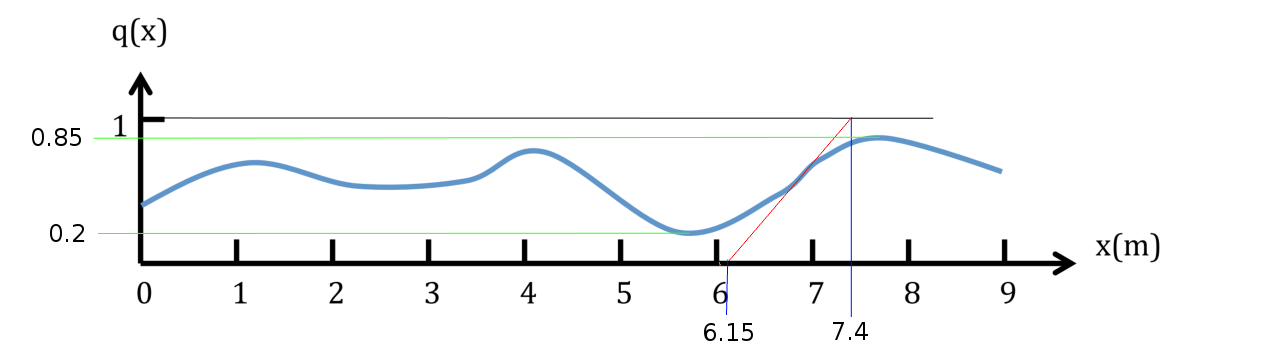
\includegraphics[scale=0.35]{./plots/3.png}
\end{center}
\end{figure}
\FloatBarrier
We find that the max amplitude of this signal is approximately 0.5(0.85 - 0.2) = 0.325 = $A_{max}$, and the max slope is $\frac{1}{7.4-6.15} =0.80 = R_{max}$. Using $R_{max} = A\omega$, we find the highest frequency to be:
\begin{equation}
\omega = \frac{R_{max}}{A} = \frac{0.8}{0.325} = 2.46
\end{equation}
We must sample at twice the frequency of the highest frequency component in order to record the signal accurately, so $\omega_{samp}$ = 2$\times$2.46 = 4.92. Therefore, maximal sampling period $X_{max}$ is:
\begin{equation}
X_{max} = \frac{2\pi}{\omega_{samp}}=\frac{2\pi}{4.92} = 1.28 \textnormal{ meters}
\end{equation}
The max sampling period is 1.3 meters.
\pagebreak
\section{Problem 4}
If any of the delta functions overlap in the Fourier transform, this means that the signal is being undersampled ($\omega_s < 2\omega_{M} $), and thus the original signal can not be recovered by from FT. This is because the signal $x(t)$ has a greater bandwidth than the spacing ($\omega_s$) between the frequencies (0, $\pm\omega_s$, $\pm2\omega_s$...) that the frequency domain "image" of the original signal is duplicated and centered at, so overlapping (superimposing) of those images (impulses) will occur. This means the frequency representation of the original signal will be corrupted, and the original signal is not deducible from it.\\\par
\section{Problem 5}
\begin{equation}
c(t) = 5e(t) + 4\int_0^te(\tau)d\tau
\label{eq:ct}
\end{equation}
\section*{a)}
If c(t) is the control signal, e(t) is the error signal, G(s) is expected to relate as follows:
\begin{equation}
C(s) = G(s)E(s) \hspace{6pt}\Rightarrow \hspace{6pt}G(s) = \frac{C(s)}{E(s)}
\end{equation}
If we take equation \ref{eq:ct} and compute the Laplace transform:
\begin{equation}
\mathcal{L}\{c(t)\} = C(s) = 5E(s) + \frac{4}{s}E(s)
\end{equation}
Now we find $\frac{C(s)}{E(s)}$
\begin{equation}
C(s) = E(s)\bigg[5 + \frac{4}{s}\bigg] \hspace{6pt}\Rightarrow \hspace{6pt} \frac{C(s)}{E(s)} = G(s) = 5 + \frac{4}{s}
\end{equation}
Therefore $G(s) =  5 + \frac{4}{s}$\\
\section*{b)}
If $ e(t) = 2e^{-4t}$, assuming for t $\geq$ 0 we find $E(s) = \frac{2}{s+4}$. We can solve for $C(s)$ in the Laplace domain easily:
\begin{equation}
C(s) = G(s)E(s) = \frac{2}{s+4}\bigg[5 + \frac{4}{s}\bigg] = \frac{10}{s+4} + \frac{8}{(s+4)s}
\end{equation}
Breaking up one of the partial fractions:
\begin{equation}
C(s) = \frac{10}{s+4} + \frac{-2}{s+4} + \frac{2}{s} = \frac{8}{s+4} + \frac{2}{s}
\end{equation}
Find $c(t)$ using inverse Laplace transform:
\begin{equation}
\mathcal{L}^{-1}\{C(s)\} = (8e^{-4t} + 2)u(t)  = c(t)
\end{equation}
Therefore $c(t) = (8e^{-4t} + 2)u(t)$ \pagebreak
\section{Problem 6}
\section*{a)}
\underline{Region 1:} poles	on the	unit	circle	correspond	to:\\
$\Rightarrow$Constant sinusoidal function \\
\underline{Region 2:} poles on the positive real axis inside the unit circle correspond to:\\ $\Rightarrow$Exponentially decaying functions\\
\underline{Region 3:} poles on the positive real axis outside the unit circle correspond to:\\ $\Rightarrow$Exponentially growing functions\\
\underline{Region 4:} pairs of complex poles inside the unit circle correspond to:\\
$\Rightarrow$Exponentially decaying sinusoidal functions\\
\underline{Region 5:} pairs of complex poles outside of the unit circle correspond to:\\
$\Rightarrow$Exponentially growing sinusoidal functions\\
\underline{Region 6:} poles on the negative real axis inside the unit circle correspond to:\\$\Rightarrow$ Exponentially decaying sinusoidal functions\\
\underline{Region 7:} poles on the negative real axis outside the unit circle correspond to:\\
$\Rightarrow$Exponentially growing sinusoidal functions\\
\section*{b)}

Region A $\Longleftrightarrow$ Region 2\\
Region B $\Longleftrightarrow$ Region 3\\
Region C $\Longleftrightarrow$ Region 1\\
Region D $\Longleftrightarrow$ Region 4 and Region 6\\
Region E $\Longleftrightarrow$ Region 5 and Region 7\\\par
\section{Problem 7}
\section*{a)}
Simplified $Human(s)$ or $H(s)$:
\begin{equation}
H(s) = k e^{-0.250s}\
\end{equation}
We can find closed loop gain $Q(s)$ knowing $H(s)$ and $S(s) = \frac{1}{s}$
\begin{equation}
Q(s) = \frac{H(s)S(s)}{1 + H(s)S(s)} = \frac{\frac{1}{s}ke^{-0.250s}}{1 +\frac{1}{s}ke^{-0.250s}}
\end{equation}
The system is unstable if $\frac{k}{s}> 1$, so we want $\frac{k}{s}= 1$ to be on the edge of stability. That means $k = s$. Therefore
\begin{equation}
Q(s) = \frac{e^{-0.250s}}{1 + e^{-0.250s}} = \frac{1}{1+e^{0.250s}}
\end{equation}
This is equivalent to a linear feedback system with H(s) being a delay system with a 250 ms delay, and the feedback G(s) = 1. So the time constant would be 250 ms from input to output.
\section*{b)}
\begin{equation}
Q(s) = \frac{e^{-2s}}{1 + e^{-2s}} = \frac{1}{1+e^{2s}}
\end{equation}
Calculations are same as before. Time constant is 2 seconds.
\section{Problem 8}
The total response $H(s)$ of $G_C(s)$, the 2x and 5x gain and $G_p(s)$ can be calculated as the product of the four. We can easily infer the s-domain functions for each looking at the given plots.
\begin{figure}[h!]
\begin{center}
 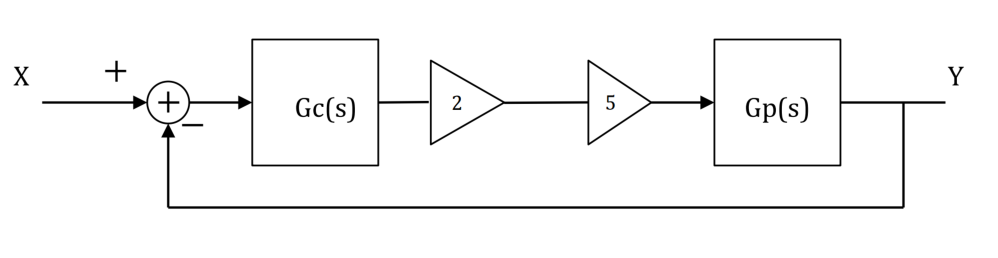
\includegraphics[scale=0.4]{./plots/g.png}
\end{center}
\end{figure}
\FloatBarrier
\begin{figure}[h!]
\begin{center}
 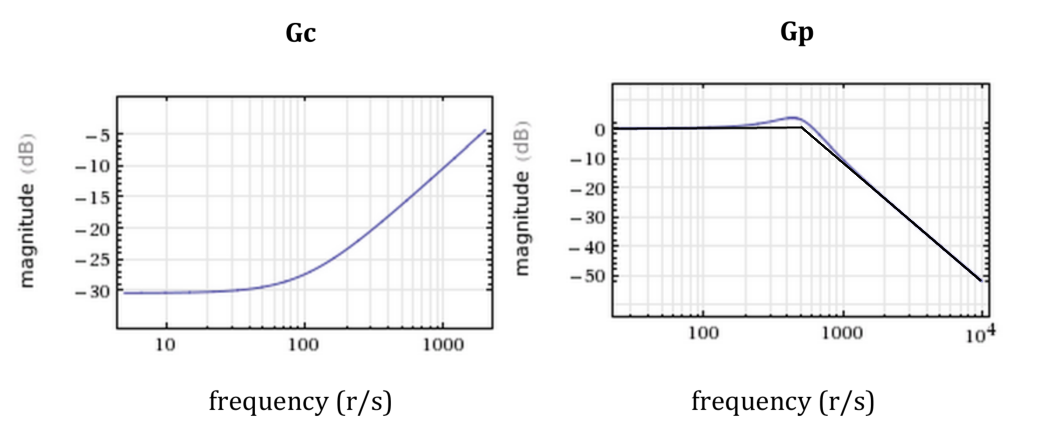
\includegraphics[scale=0.4]{./plots/f.png}
\end{center}
\end{figure}
\FloatBarrier
$G_C(s)$ looks like a single zero filter (because it rises at +20dB per decade after the corner) with a DC gain of -30 dB, or A = $10^{-1.5}$, and the corner frequency occurring at 100 r/s. This gives a $G_C(s)$ of:
\begin{equation}
G_C(s)=10^{-1.5}(1+\frac{s}{100})
\end{equation}
$G_P(s)$ looks like a second order damped system (decreasing after the corner at -40 dB per decade), with a DC gain of 0 dB, or A = 1, and a corner frequency of 500 r/s found using a straight line approximation. $\zeta \approx 0.4$, based upon figures given in the textbook. This means $G_P(s)$ is:
\begin{equation}
G_P(s) =\frac{1}{\big(\frac{s}{\omega_n}\big)^2+2\zeta\big(\frac{s}{\omega_n}\big)+1} =\frac{1}{\big(\frac{s}{500}\big)^2+0.8\big(\frac{s}{500}\big)+1}
\end{equation}
Therefore $H(s)$ is the product of these responses:
\begin{equation}
H(s) = \frac{10* 10^{-1.5}(1+\frac{s}{100})}{\big(\frac{s}{500}\big)^2+0.8\big(\frac{s}{500}\big)+1}= \frac{10^{-0.5}(1+\frac{s}{100})}{\big(\frac{s}{500}\big)^2+0.8\big(\frac{s}{500}\big)+1}
\end{equation}
The closed loop transfer function of the system is:
\begin{equation}
Q(s) = \frac{H(s)}{1+H(s)} = \frac{\frac{10^{-0.5}(1+\frac{s}{100})}{\big(\frac{s}{500}\big)^2+0.8\big(\frac{s}{500}\big)+1}}{1 + \frac{10^{-0.5}(1+\frac{s}{100})}{\big(\frac{s}{500}\big)^2+0.8\big(\frac{s}{500}\big)+1}} = \frac{10^{-0.5}(1+\frac{s}{100})}{10^{-0.5}(1+\frac{s}{100}) + \big(\frac{s}{500}\big)^2+0.8\big(\frac{s}{500}\big)+1}
\end{equation}
%From $Q(s)$ we can find $\lvert Q(\omega) \rvert$ to figure out the bandwidth:
%\begin{equation}
%\lvert Q(\omega) \rvert = \sqrt{\frac{10^{-5}\omega^2 + 10^{-10}}{\big(1 + 10^{-5} - %\frac{\omega^2}{500^2}\big)^2+\omega^2\big(\frac{0.8}{500}+10^{-2.5}\big)^2}}
%\end{equation}
Here is the Bode diagram of this closed loop response from Wolfram:
\begin{figure}[h!]
\begin{center}
 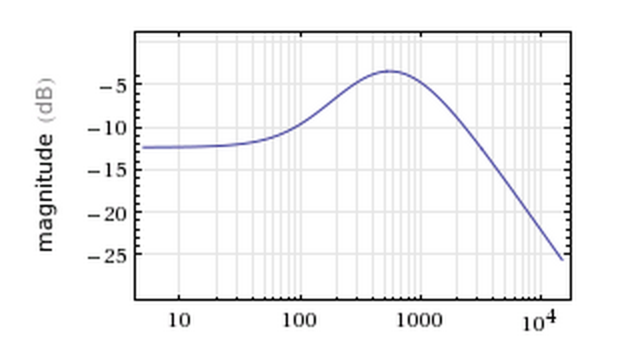
\includegraphics[scale=0.4]{./plots/s.png}
\end{center}
\end{figure}
\FloatBarrier
The Maxima of the transfer function is at 500 r/s, with a gain of -3.56 dB, and the DC gain is -12.39 dB. The bandwidth of this system can be classified in two ways, one viewing it as a low pass filter and considering the cutoff/bandwidth to be -3 dB from the DC value, and the second seeing it as a sort of band pass filter and the bandwidth being the difference between the two -3dB points relative to the peak. The low pass filter bandwidth was found to be 4.58 kHz (AKA $\omega_{cutoff}$ using the Bode plot) at -3 dB from the DC gain. The Band pass bandwidth was found to be 1.12 - 0.200 = 0.92 kHz.\\\par

Therefore, the "Lowpass" bandwidth is 4.58 kHz and the "Bandpass" bandwidth is 0.92 kHz.
\end{document}